% Options for packages loaded elsewhere
\PassOptionsToPackage{unicode}{hyperref}
\PassOptionsToPackage{hyphens}{url}
%
\documentclass[
]{book}
\usepackage{lmodern}
\usepackage{amssymb,amsmath}
\usepackage{ifxetex,ifluatex}
\ifnum 0\ifxetex 1\fi\ifluatex 1\fi=0 % if pdftex
  \usepackage[T1]{fontenc}
  \usepackage[utf8]{inputenc}
  \usepackage{textcomp} % provide euro and other symbols
\else % if luatex or xetex
  \usepackage{unicode-math}
  \defaultfontfeatures{Scale=MatchLowercase}
  \defaultfontfeatures[\rmfamily]{Ligatures=TeX,Scale=1}
\fi
% Use upquote if available, for straight quotes in verbatim environments
\IfFileExists{upquote.sty}{\usepackage{upquote}}{}
\IfFileExists{microtype.sty}{% use microtype if available
  \usepackage[]{microtype}
  \UseMicrotypeSet[protrusion]{basicmath} % disable protrusion for tt fonts
}{}
\makeatletter
\@ifundefined{KOMAClassName}{% if non-KOMA class
  \IfFileExists{parskip.sty}{%
    \usepackage{parskip}
  }{% else
    \setlength{\parindent}{0pt}
    \setlength{\parskip}{6pt plus 2pt minus 1pt}}
}{% if KOMA class
  \KOMAoptions{parskip=half}}
\makeatother
\usepackage{xcolor}
\IfFileExists{xurl.sty}{\usepackage{xurl}}{} % add URL line breaks if available
\IfFileExists{bookmark.sty}{\usepackage{bookmark}}{\usepackage{hyperref}}
\hypersetup{
  pdftitle={A tutorial for geochemical modeling of fluid-rock interaction using GEM-Selektor and the MINES thermodynamic database},
  pdfauthor={Alexander Gysi},
  hidelinks,
  pdfcreator={LaTeX via pandoc}}
\urlstyle{same} % disable monospaced font for URLs
\usepackage{longtable,booktabs}
% Correct order of tables after \paragraph or \subparagraph
\usepackage{etoolbox}
\makeatletter
\patchcmd\longtable{\par}{\if@noskipsec\mbox{}\fi\par}{}{}
\makeatother
% Allow footnotes in longtable head/foot
\IfFileExists{footnotehyper.sty}{\usepackage{footnotehyper}}{\usepackage{footnote}}
\makesavenoteenv{longtable}
\usepackage{graphicx,grffile}
\makeatletter
\def\maxwidth{\ifdim\Gin@nat@width>\linewidth\linewidth\else\Gin@nat@width\fi}
\def\maxheight{\ifdim\Gin@nat@height>\textheight\textheight\else\Gin@nat@height\fi}
\makeatother
% Scale images if necessary, so that they will not overflow the page
% margins by default, and it is still possible to overwrite the defaults
% using explicit options in \includegraphics[width, height, ...]{}
\setkeys{Gin}{width=\maxwidth,height=\maxheight,keepaspectratio}
% Set default figure placement to htbp
\makeatletter
\def\fps@figure{htbp}
\makeatother
\setlength{\emergencystretch}{3em} % prevent overfull lines
\providecommand{\tightlist}{%
  \setlength{\itemsep}{0pt}\setlength{\parskip}{0pt}}
\setcounter{secnumdepth}{5}
\usepackage{booktabs}
\usepackage{amsthm}
\makeatletter
\def\thm@space@setup{%
  \thm@preskip=8pt plus 2pt minus 4pt
  \thm@postskip=\thm@preskip
}
\makeatother
\usepackage[]{natbib}
\bibliographystyle{apalike}

\title{A tutorial for geochemical modeling of fluid-rock interaction using GEM-Selektor and the MINES thermodynamic database}
\author{Alexander Gysi}
\date{2020-12-01}

\begin{document}
\maketitle

{
\setcounter{tocdepth}{1}
\tableofcontents
}
\hypertarget{prerequisites}{%
\chapter*{Prerequisites}\label{prerequisites}}
\addcontentsline{toc}{chapter}{Prerequisites}

GEM-Selektor (GEMS), is a numerical modeling program with a graphical user interface based on Gibbs energy minimization and permits calculating and solving fluid-rock interaction problems of interest in geochemistry.

\begin{itemize}
\item
  Installation instructions for GEMS and more information about this modeling program can be found on the GEMS team webpage: \url{http://gems.web.psi.ch/GEMS3/techinfo.html}.
\item
  Information about the MINES database and project files for the tutorials can be found under \url{https://geoinfo.nmt.edu/tdb-mines}
\end{itemize}

This booklet is subdivided into five modules.

\begin{itemize}
\tightlist
\item
  Module 1: Create your first project in GEMS and installing the MINES database
\end{itemize}

\hypertarget{intro}{%
\chapter{Create your first project in GEMS}\label{intro}}

Here we will learn how to create a new Project, the selection of thermodynamic databases, components and equations of state for your modeling project. We will also explain the project folder structure and how to install the \href{https://geoinfo.nmt.edu/mines-tdb}{MINES thermodynamic database} for modeling hydrothermal fluid-rock interaction and ore-forming processes . You will also learn how to interact basalt with water in your first equilibrium calculations.

\hypertarget{installing-the-mines-thermodynamic-database}{%
\section{Installing the MINES thermodynamic database}\label{installing-the-mines-thermodynamic-database}}

The MINES thermodynamic database can be downloaded at \url{https://geoinfo.nmt.edu/tdb} (Fig. \ref{fig:fig-1}).

\begin{figure}
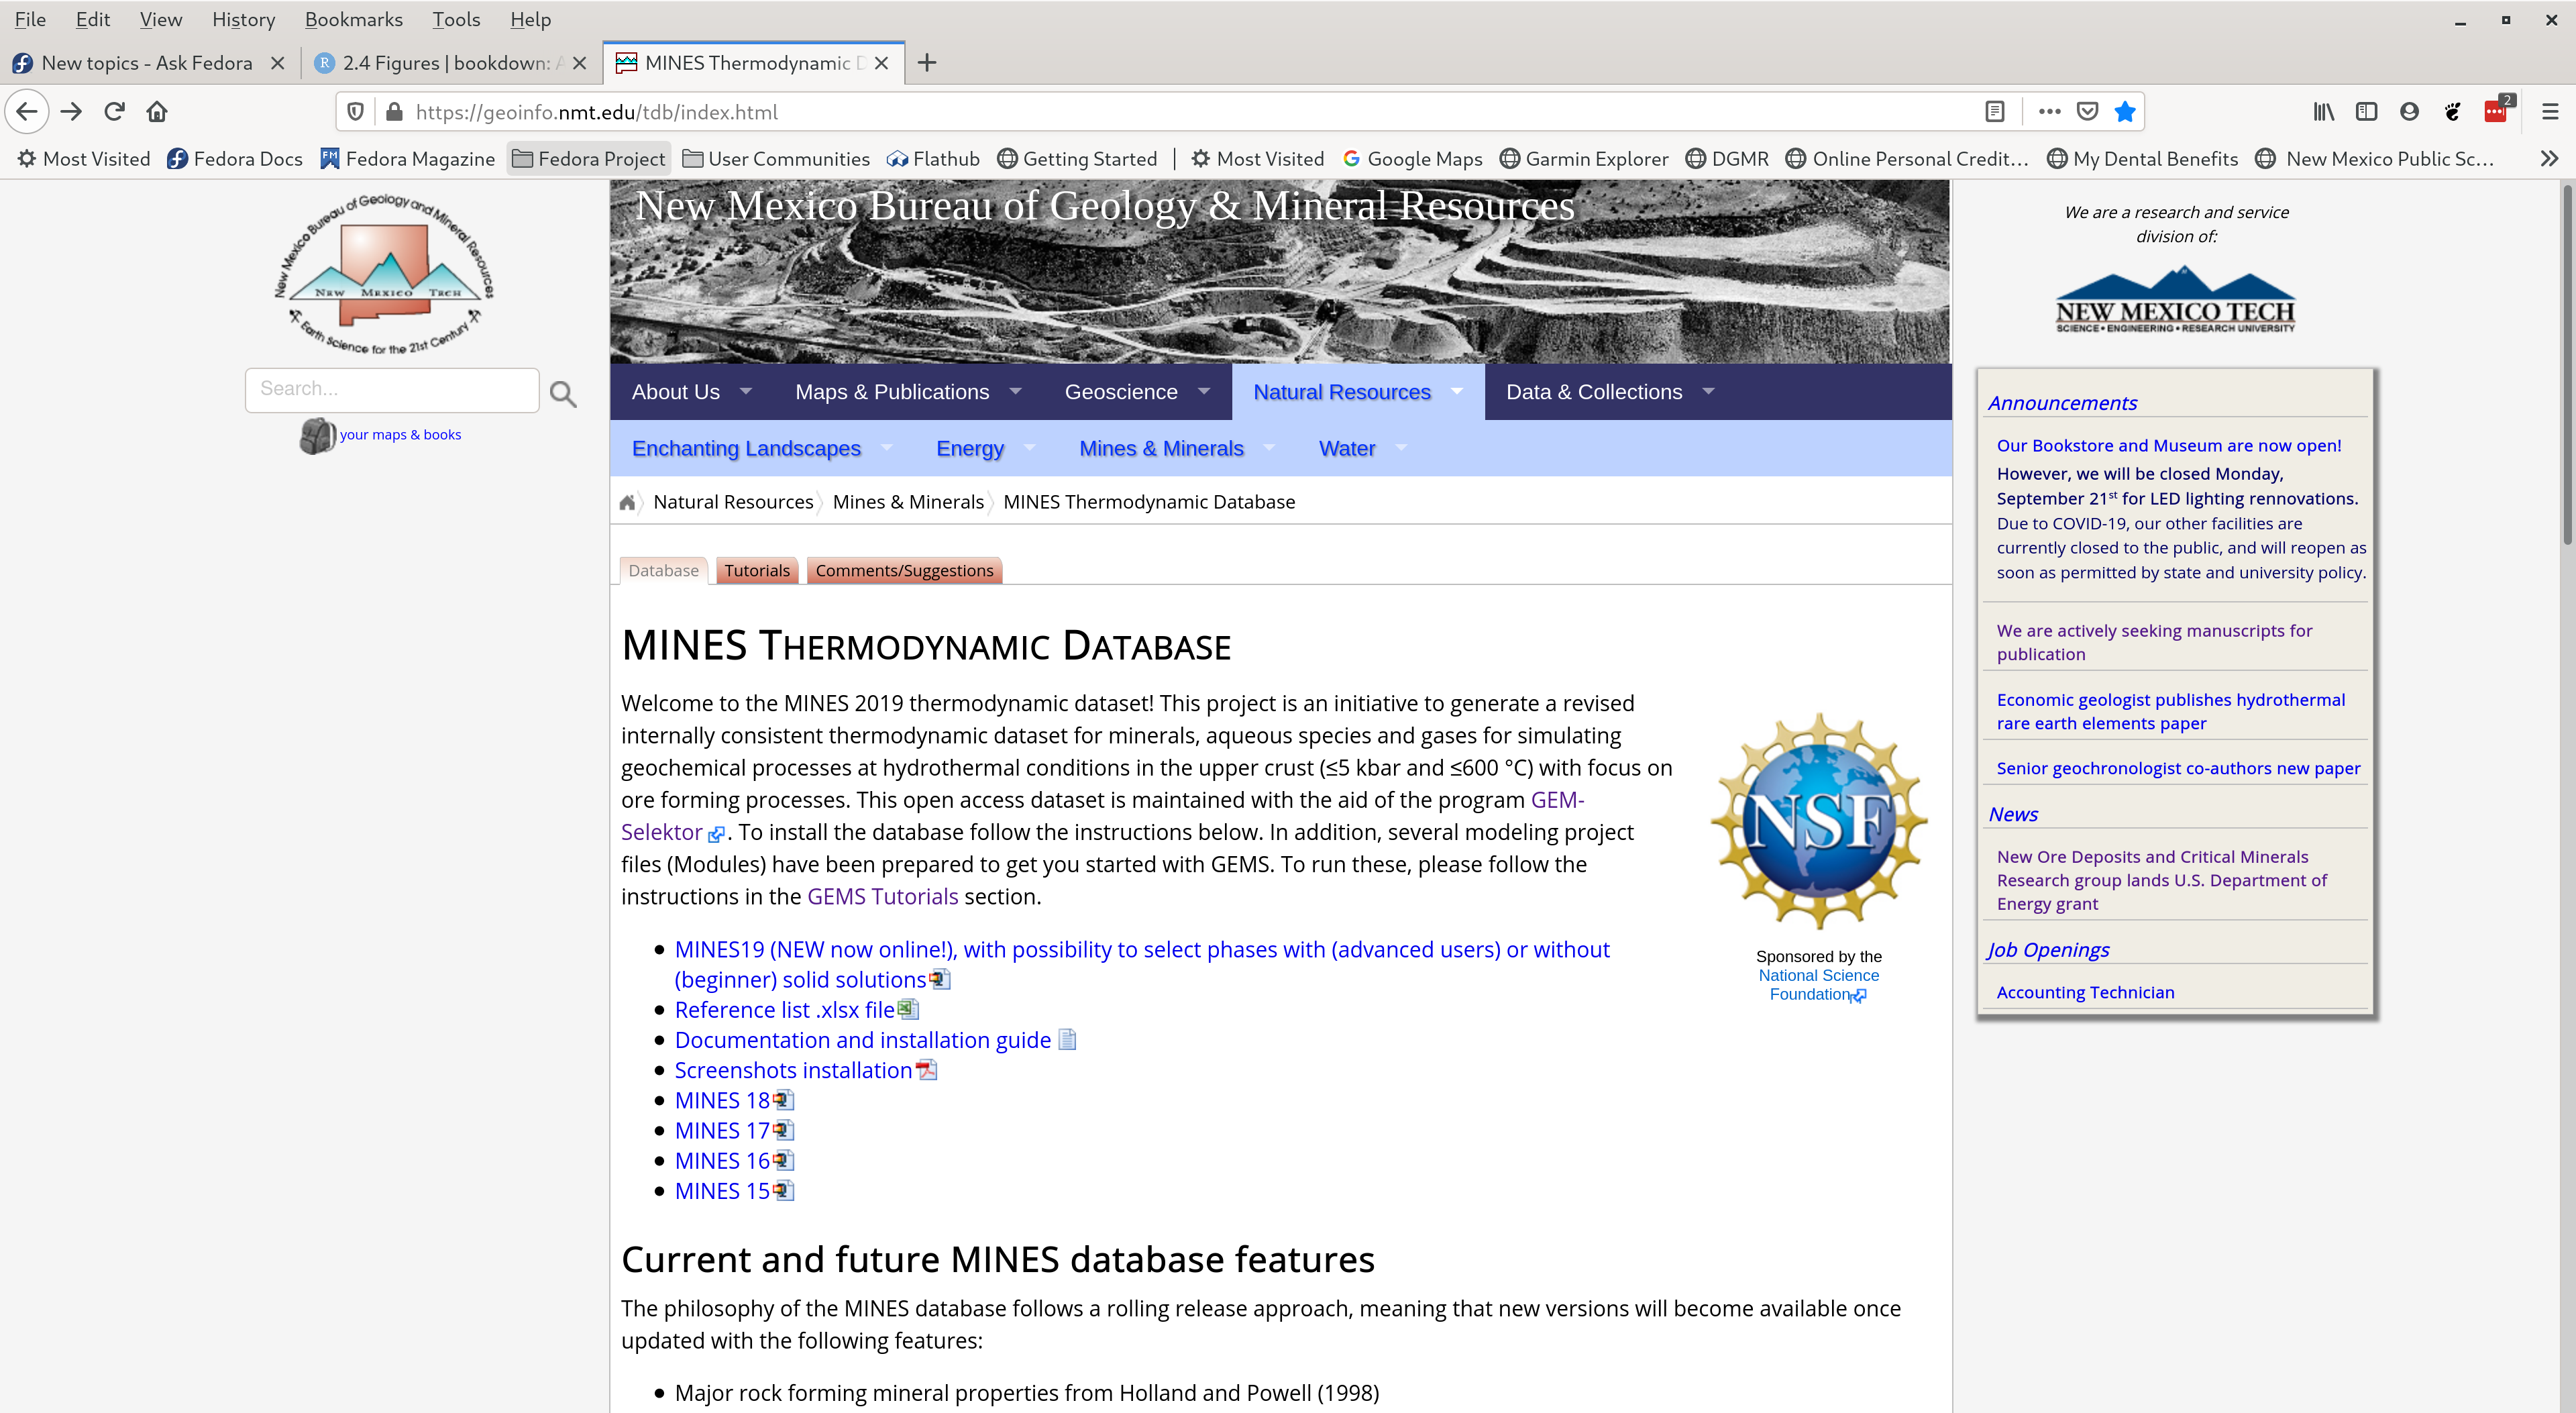
\includegraphics[width=0.9\linewidth]{figures/module1/fig-1} \caption{The MINES thermodynamic database webpage and files to download. Select the weblink for MINES19.}\label{fig:fig-1}
\end{figure}

\begin{itemize}
\item
  Download and unzip the DB19.default archive folder to Downloads. Select all the database files in this folder and copy them (Fig. \ref{fig:fig-2}).
\item
  Merge these database files with the Gems3-app/Resources/DB.default folder by pasting them into DB.default (Fig. \ref{fig:fig-3}).
\end{itemize}

\emph{In Linux this folder is in /Gems3-app/Resources/DB.default; In Mac OSX this folder is in /Applications/gems3 then right-click show package content and go to Contents/Resources/DB.default; In Windows this folder should be in /Gems3-app/Resources/DB.default.}

The folder structure of the GEMS program, independent of the operating system used, consists of two main folders:

\begin{itemize}
\tightlist
\item
  Gems3-app

  \begin{itemize}
  \tightlist
  \item
    The GEMS3-app folder contains the program resources and also a subfolder Resources/ DB.default, which will be used to copy the MINES thermodynamic database files into it.
  \end{itemize}
\item
  Library/Gems3/projects

  \begin{itemize}
  \tightlist
  \item
    The projects folder will contain all the projects you create and work on, and will also be the folder in which you can copy the tutorial folders.
  \end{itemize}
\end{itemize}

\begin{figure}
 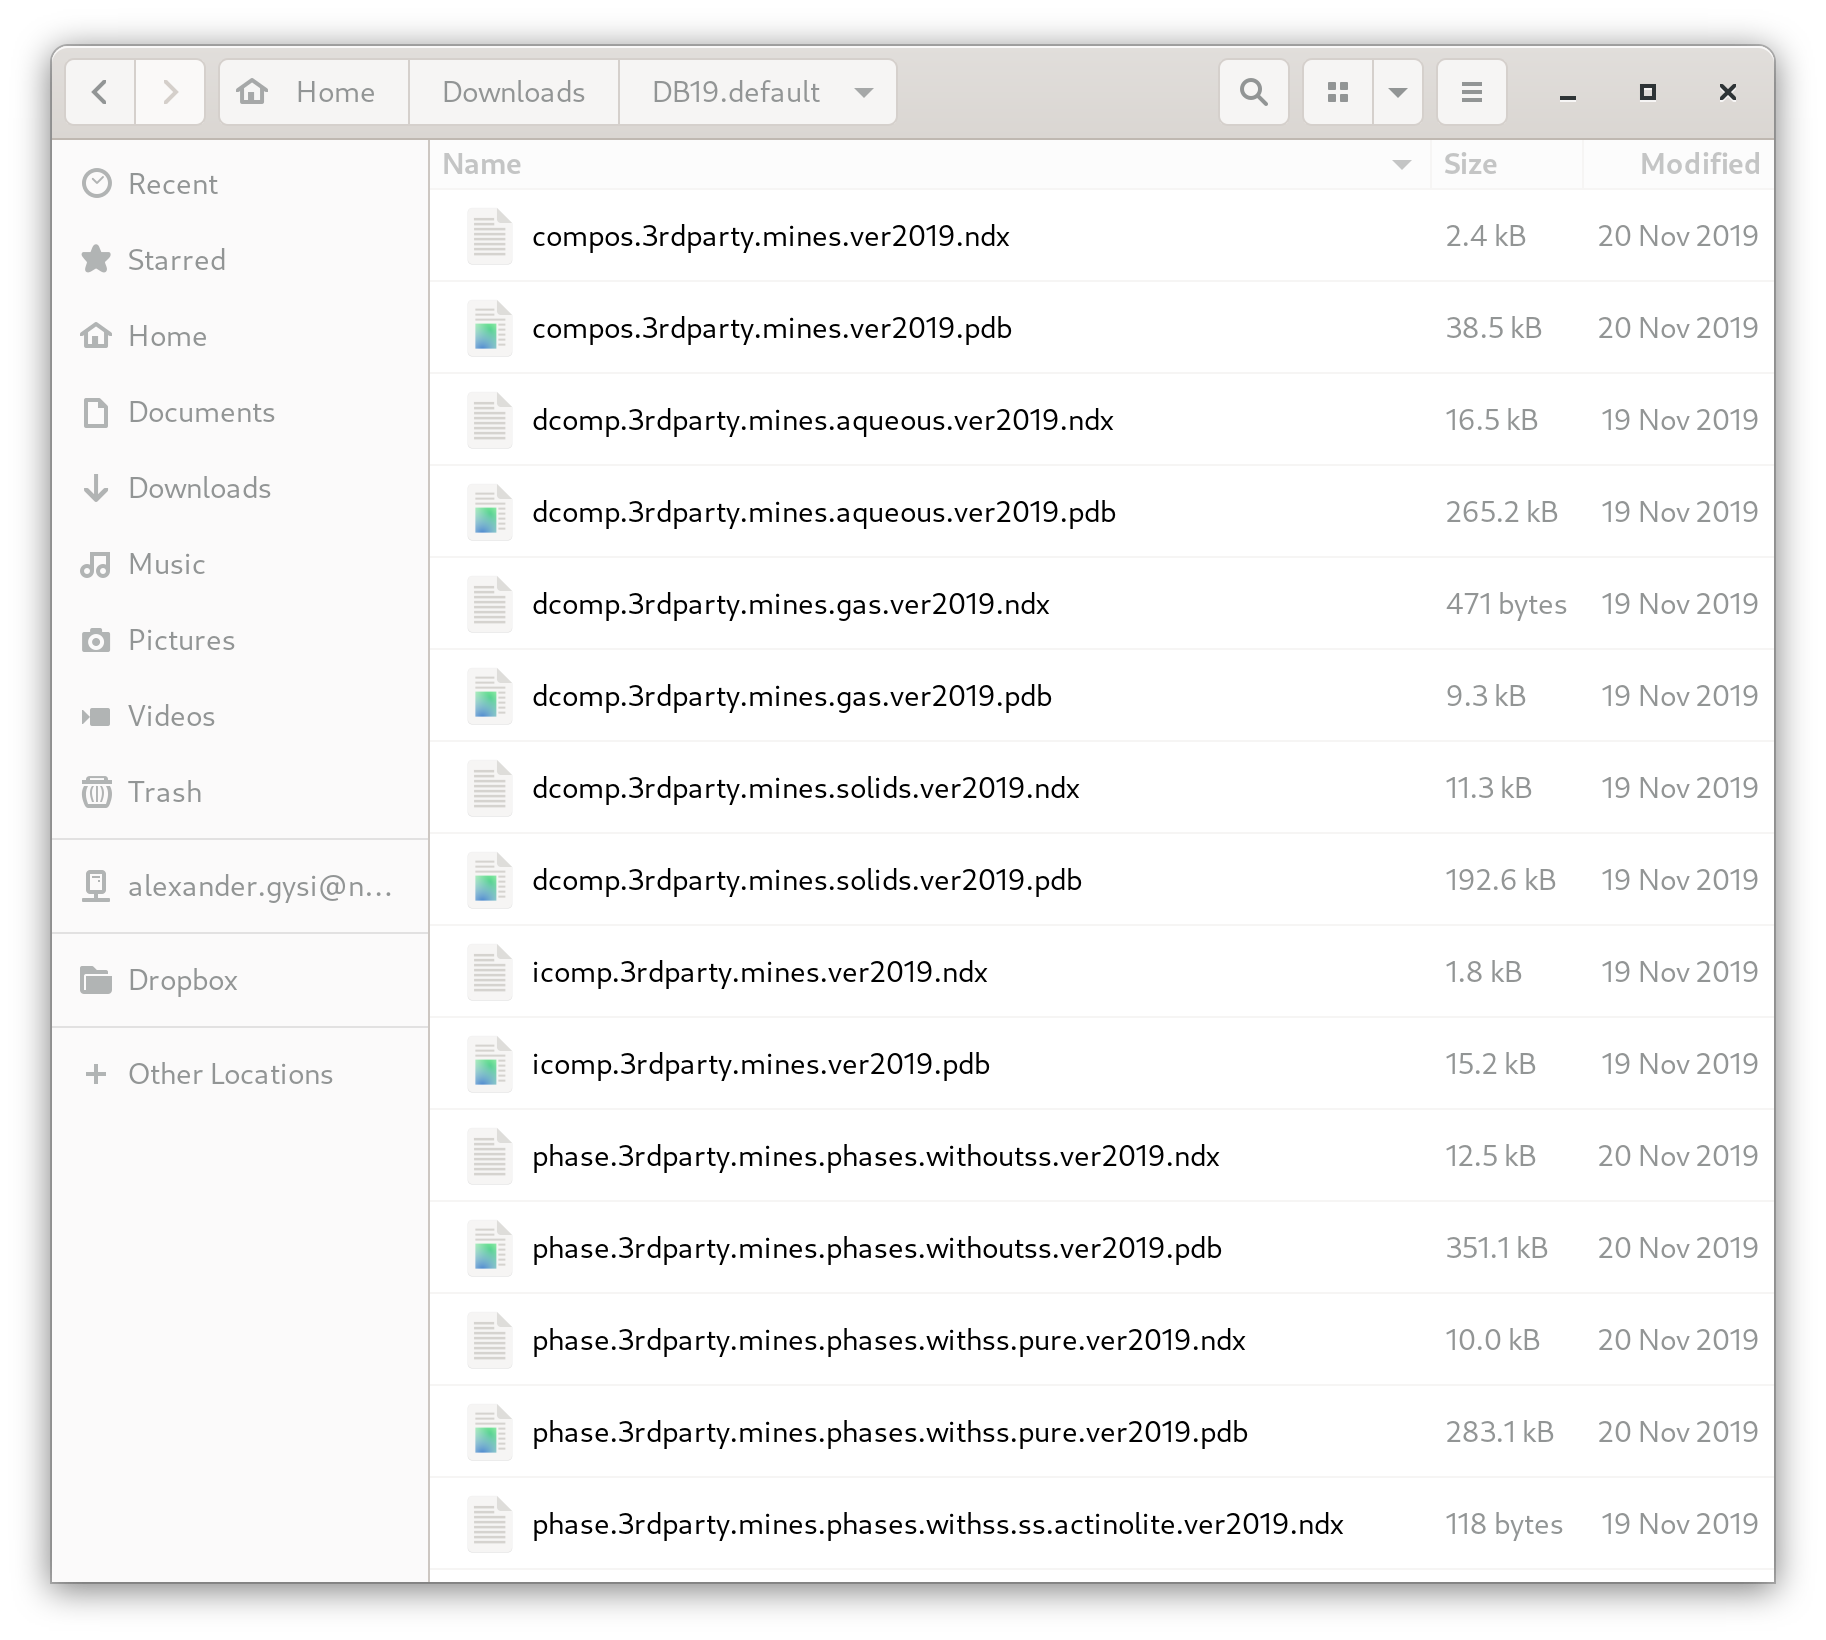
\includegraphics[width=0.7\linewidth]{figures/module1/fig-2} \caption{Unzipped DB19.default folder and database files to copy.}\label{fig:fig-2}
 \end{figure}

\begin{figure}
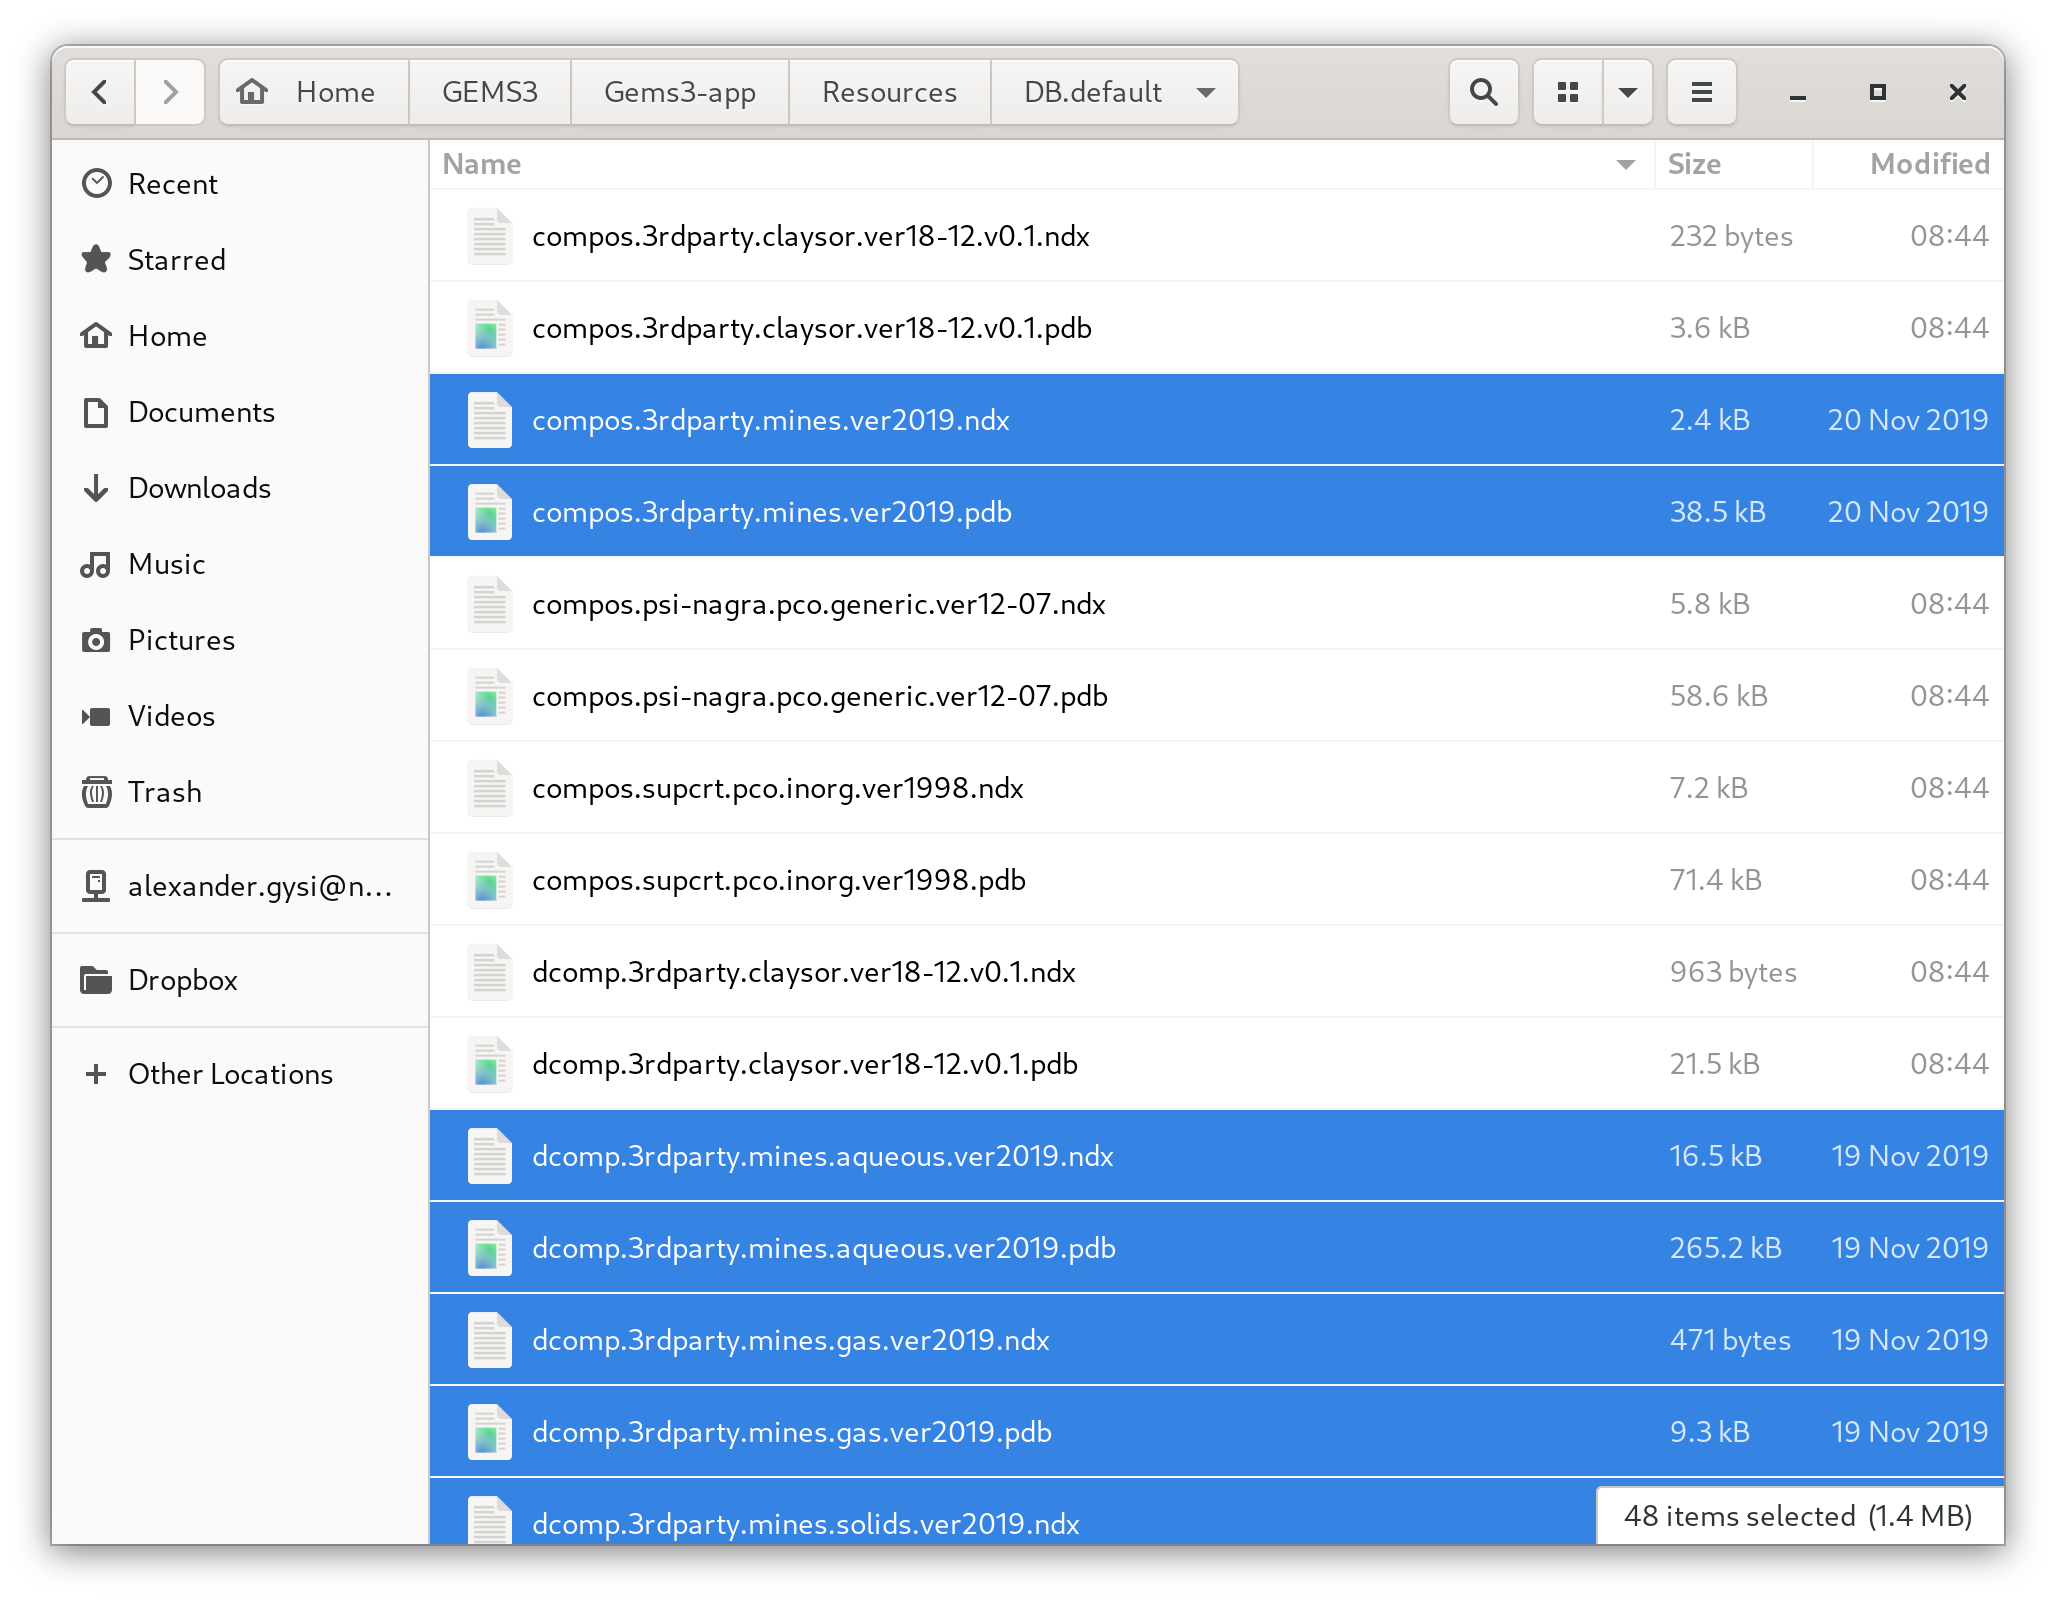
\includegraphics[width=0.7\linewidth]{figures/module1/fig-3} \caption{Database files merged with the Gems3-app/Resources/DB.default folder in GEMS.}\label{fig:fig-3}
\end{figure}

\hypertarget{creating-a-new-project-from-scratch}{%
\section{Creating a new project from scratch}\label{creating-a-new-project-from-scratch}}

\begin{itemize}
\item
  Open GEMS and click \texttt{New\ Project} in the Modeling Projects window. Give a name to your project (no spaces). The user interface is shown in Figure \ref{fig:fig-4}.
\item
  In the next window, you can choose the thermodynamic database for your project. Select the database files 3rdparty/MINES and support, then deselect other databases as shown in Figure \ref{fig:fig-5}. Click \texttt{Next}.
\end{itemize}

\emph{Do not forget, you have an extensive list of minerals included in this database. Once you have gone through the tutorials and are familiar with GEMS, it is suggested that in thermodynamic database mode you switch to the \texttt{Phase} module (Fig. \ref{fig:fig-9}), and remove minerals that are not relevant for your own specific project. Also, for less advanced users, it is easiedt to not use the ternary non-ideal feldspar solid solution model (ss) but only their end members (i.e., anorthite, albite and microcline).}

\begin{figure}
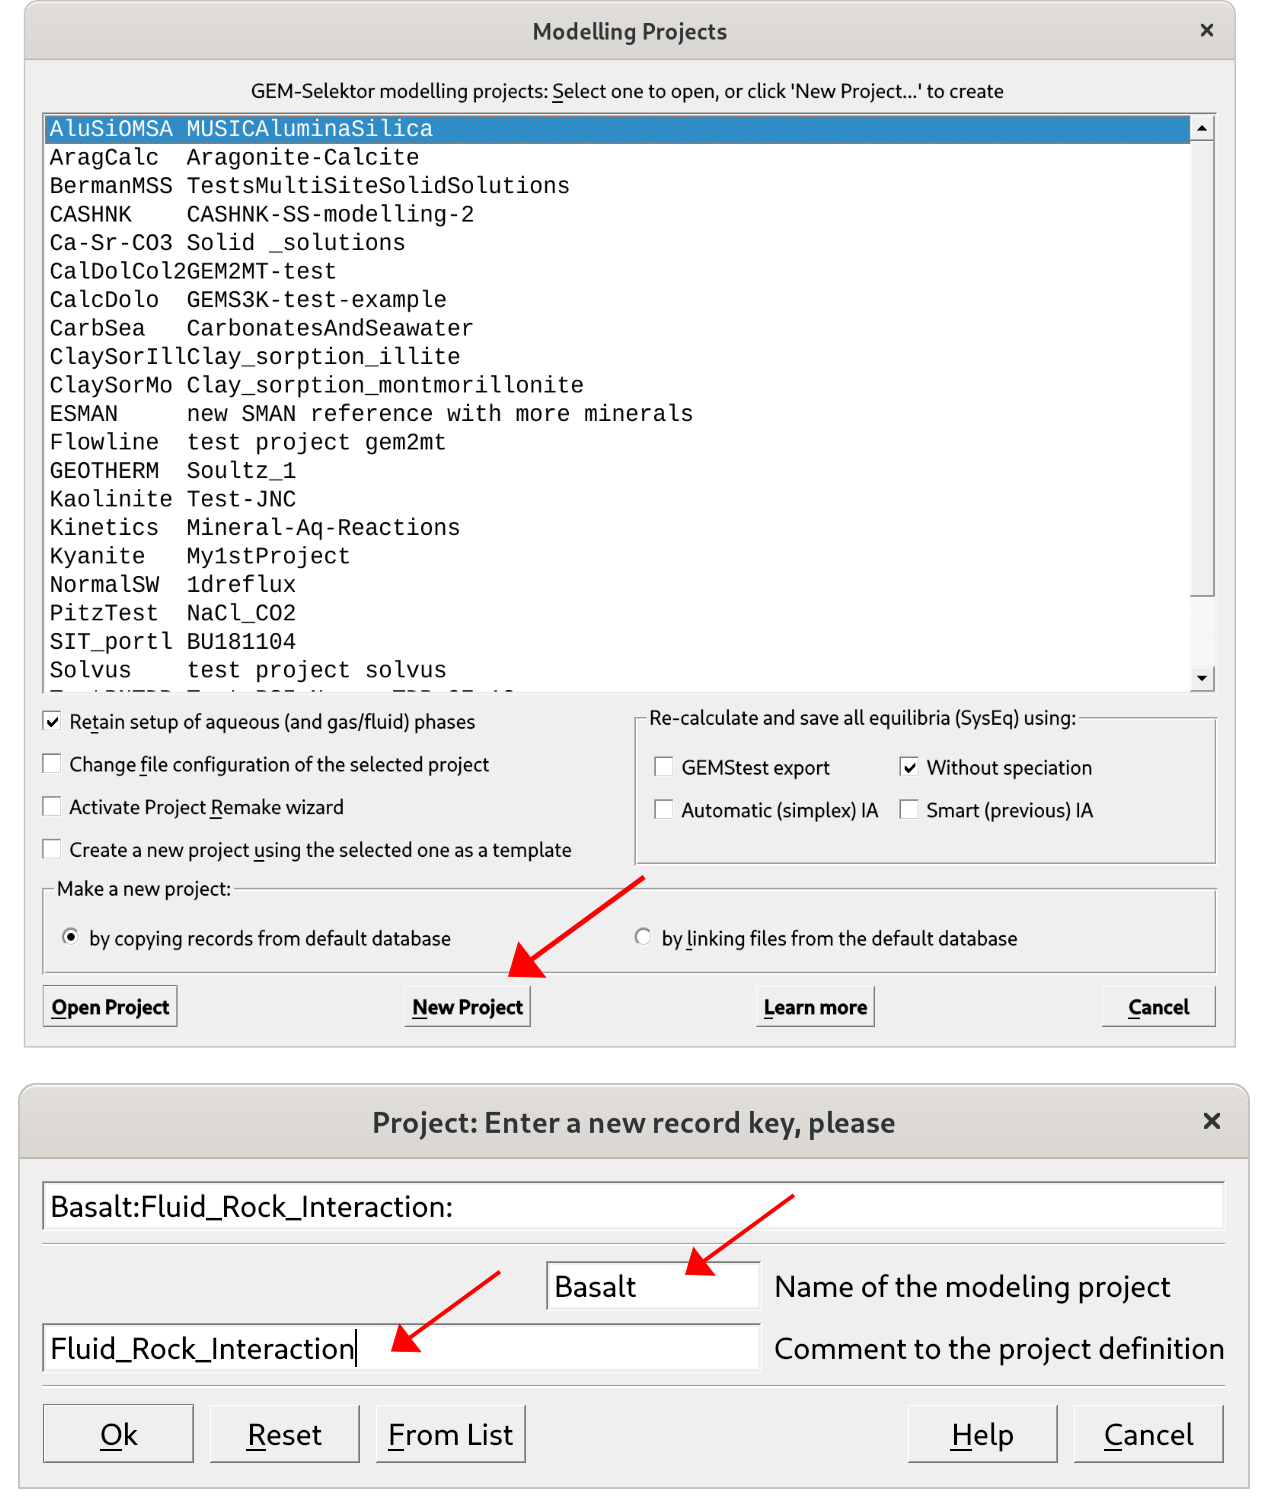
\includegraphics[width=0.7\linewidth]{figures/module1/fig-4} \caption{GEMS user interface showing the project window. Click on make a `New Project` and select a project name without spaces.}\label{fig:fig-4}
\end{figure}

\textbackslash begin\{figure\}
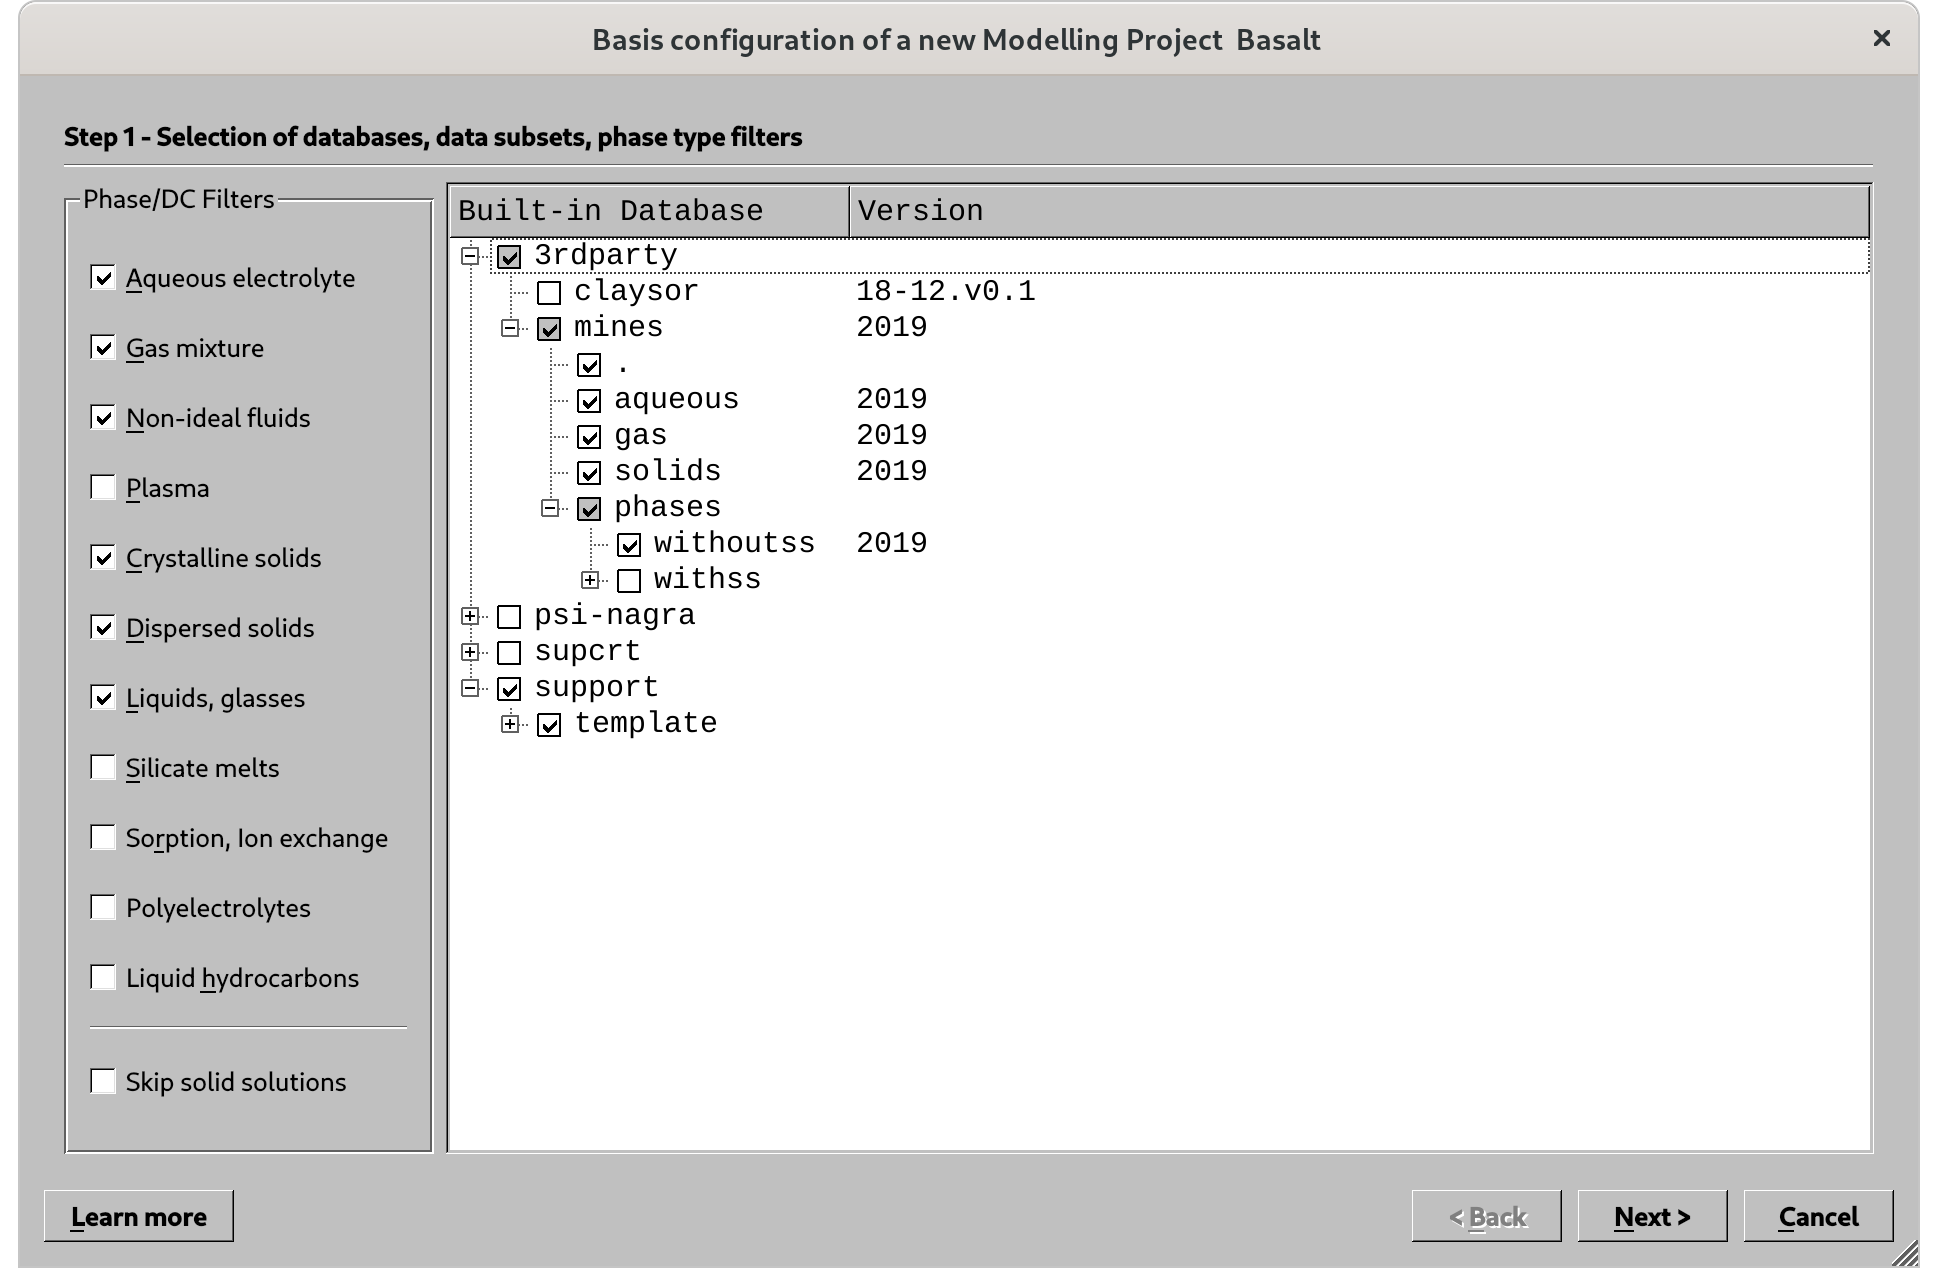
\includegraphics[width=0.7\linewidth]{figures/module1/fig-5} \textbackslash caption\{Select 3rdparty/mines and support, and for phases select only withoutss. \emph{Note that we recommend only advanced users to choose withss; the expanded tab shows pure for endmembers and ss for different solid solution endmembers}\}\label{fig:fig-5}
\textbackslash end\{figure\}

\begin{itemize}
\item
  In the next window choose your system components: H-O-C-Cl-Na-K-Ca-Mg-Al-Fe-Si-Ti (Fig. \ref{fig:fig-6}). Have you checked you got all of the elements selected? Check again please, then click \texttt{Next}\ldots By doing so, GEMS will automatically look up all phases with these components in the MINES database and copy them into your modeling project! \emph{Tip of the day: all your modeling projects you are working on are located under Library/Gems3/projects. Make sure to do regular backups\ldots{}}
\item
  In the next window you will be able to choose the activity model for your aqueous speciation calculations (e.g.~``Debye-Hückel'', Davies equation, \ldots), and the EOS for gases. For now, follow Figure \ref{fig:fig-7} using the extended ``Debye-Hückel'' equation (Helgeson), check the parameters and click \texttt{Check} for the aqueous speciation model. \emph{This model is ideal for modeling H\(_2\)O-NaCl aqueous solutions (with NaCl as background electrolyte) at hydrothermal conditions at relatively moderate salinities observed in many ore deposits.}
\item
  Then you can switch to the gas EOS model tab and choose the Peng-Robinson-Stryjek-Vera (PRSV) model and click \texttt{Check} (Fig. \ref{fig:fig-7}). That's it, now you are ready to model your first equilibrium model!
\end{itemize}

\emph{Note: this model is for non-ideal gases, and for this purpose a new phase with the acronym (f) was added to the MINES database with all the relevant parameters using the PRSV EOS. Else the choice would be the ideal gas law with a phase using the acronym (g)}

\begin{figure}
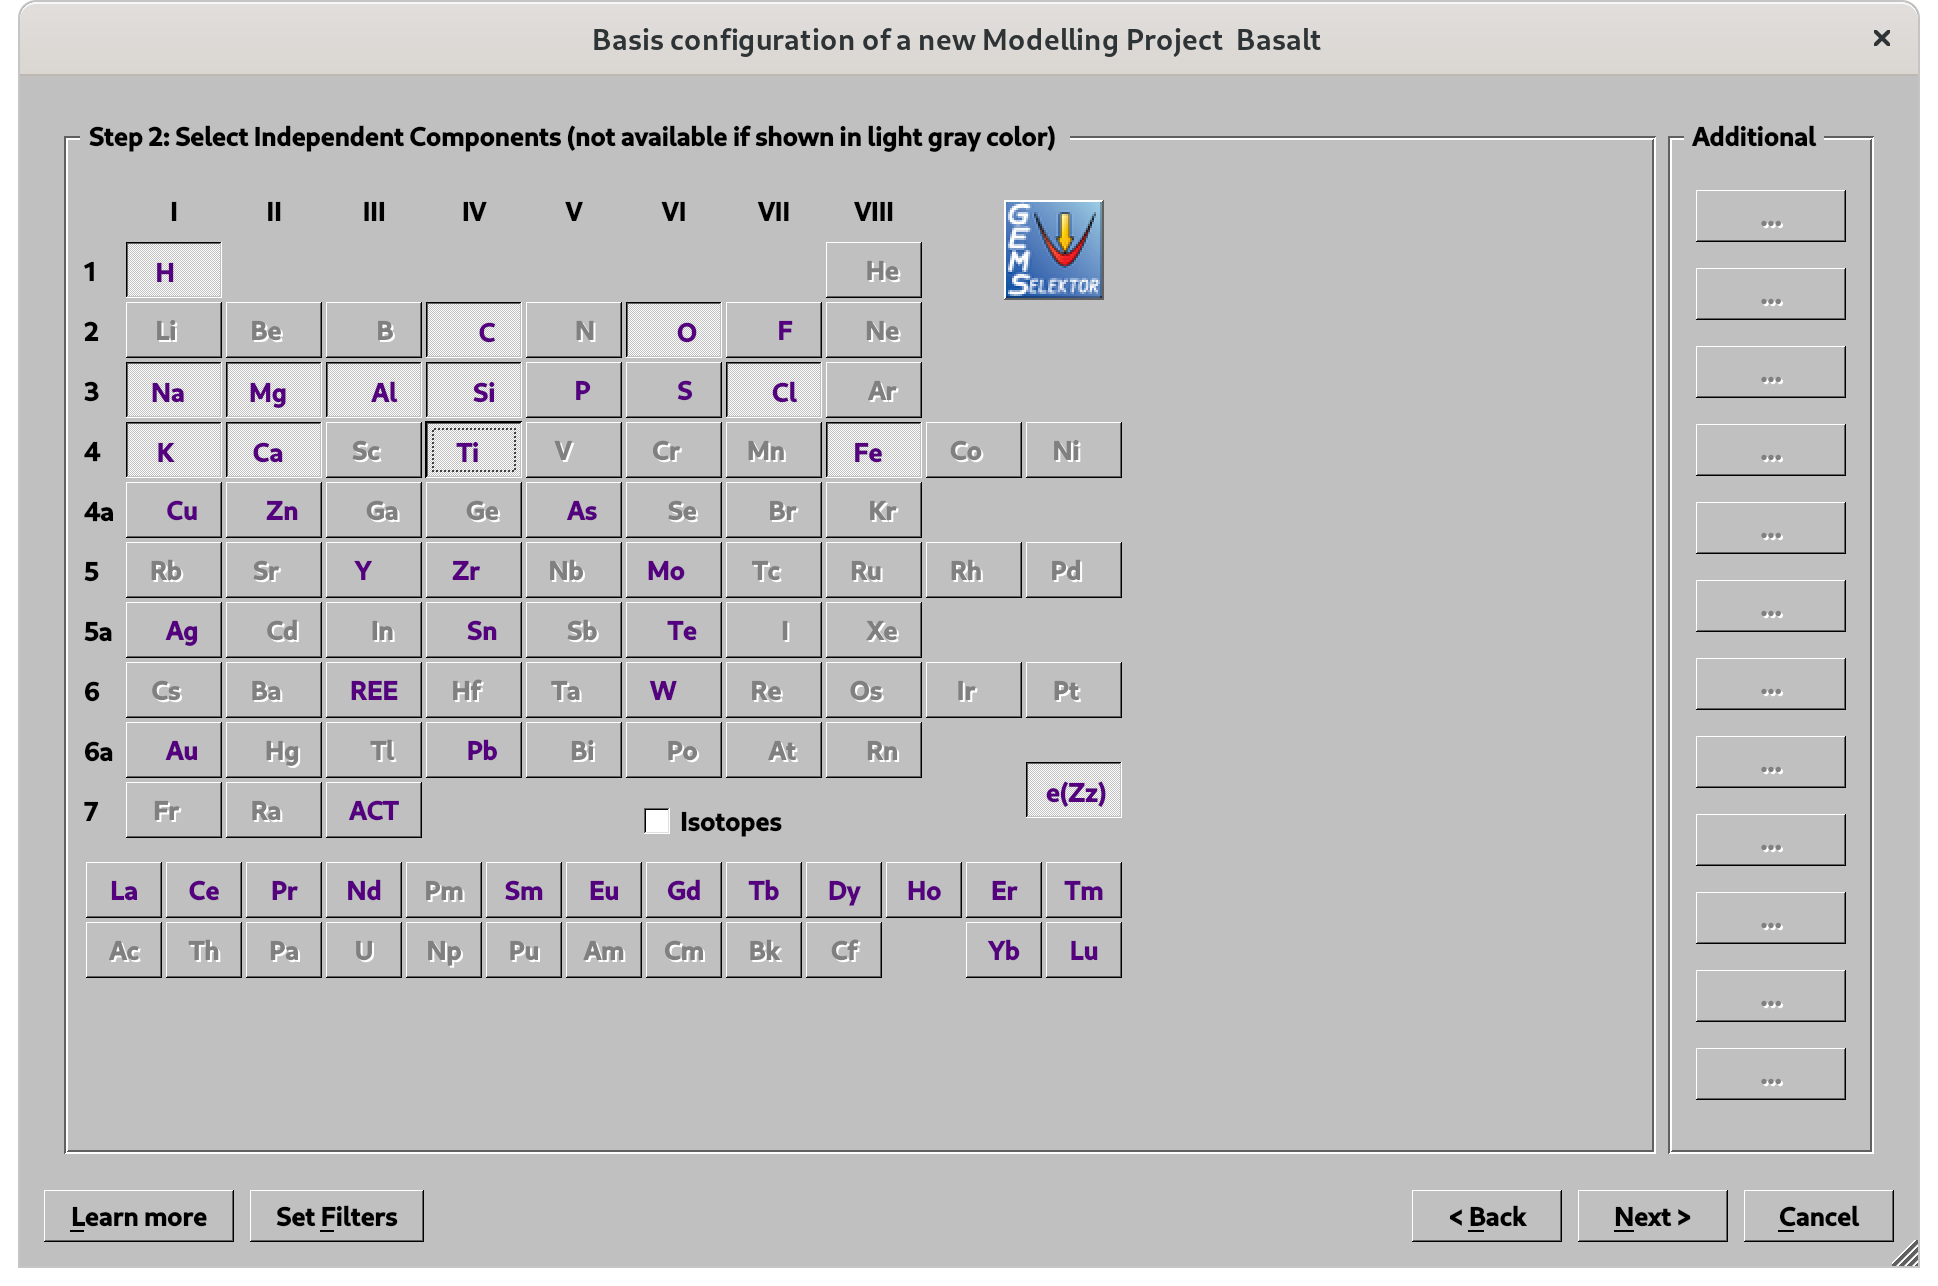
\includegraphics[width=0.8\linewidth]{figures/module1/fig-6} \caption{Select here the composition of the system. All phases containing these elements will automatically be loaded from the MINES database into your project.}\label{fig:fig-6}
\end{figure}

\begin{figure}
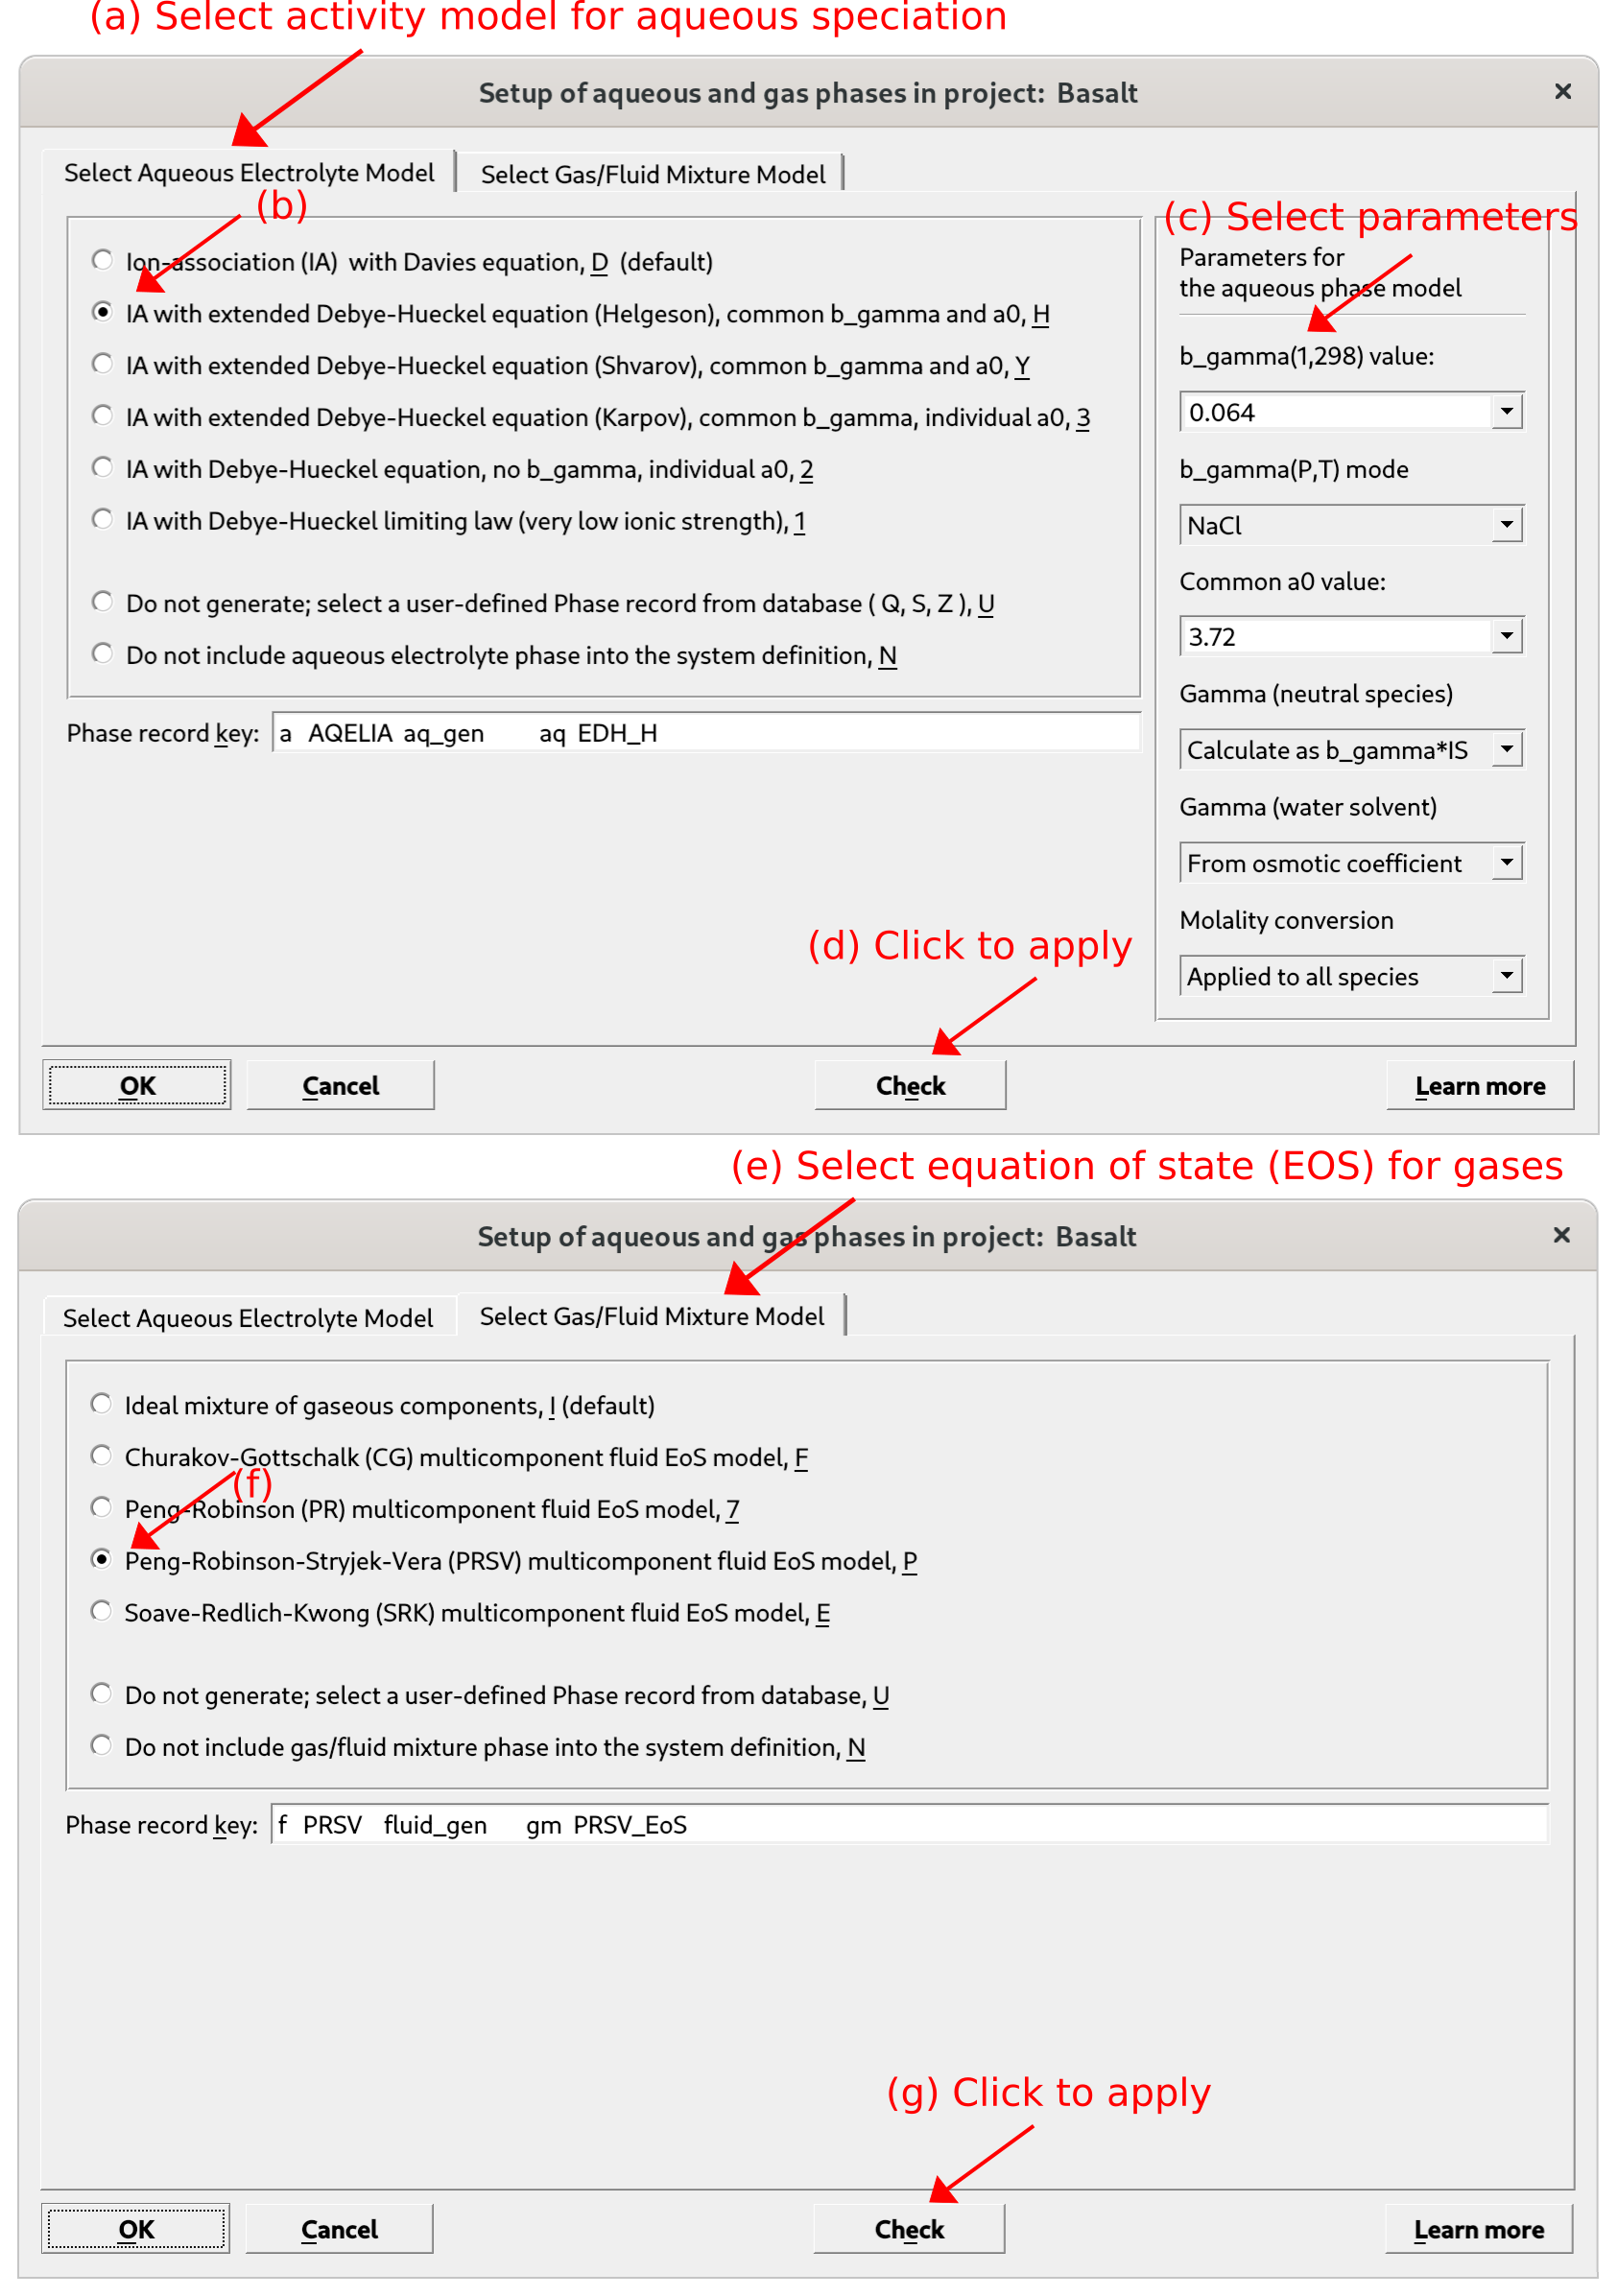
\includegraphics[width=0.7\linewidth]{figures/module1/fig-7} \caption{Select here the activity model for aqueous speciation (a-d) and the EOS model for gases (e-g).}\label{fig:fig-7}
\end{figure}

\hypertarget{your-first-fluid-rock-equilibrium-model}{%
\section{Your first fluid-rock equilibrium model}\label{your-first-fluid-rock-equilibrium-model}}

\begin{itemize}
\item
  In the next window, you will be able to define the name of your first fluid-rock system equilibrium (\texttt{SysEq}) calculations and set the pressure and temperature (Fig. \ref{fig:fig-8}).
\item
  Add a name without spaces and P-T conditions, i.e.~we choose basalt-fluid, 250 \(^{\circ}\)C for T and 1 kbar for P.
\item
  Next window we select our ingredients and add 1000 g of H\(_2\)O (Aqua), 200 g of NaCl, 5 g Gas CO\(_2\) and 500 g of basalt (Fig. \ref{fig:fig-8}). Click \texttt{OK}.
\item
  Finally, you can click on \texttt{Calculate\ BCC} followed by \texttt{Calculate\ equilibrium\ with\ GEM} as shown in (Fig. \ref{fig:fig-9}). You can easily create another system by selecting \texttt{Clone\ a\ new\ record\ from\ this\ one} and change the fluid/rock ratio or temperature and see what what happens with the results.
\end{itemize}

\begin{figure}
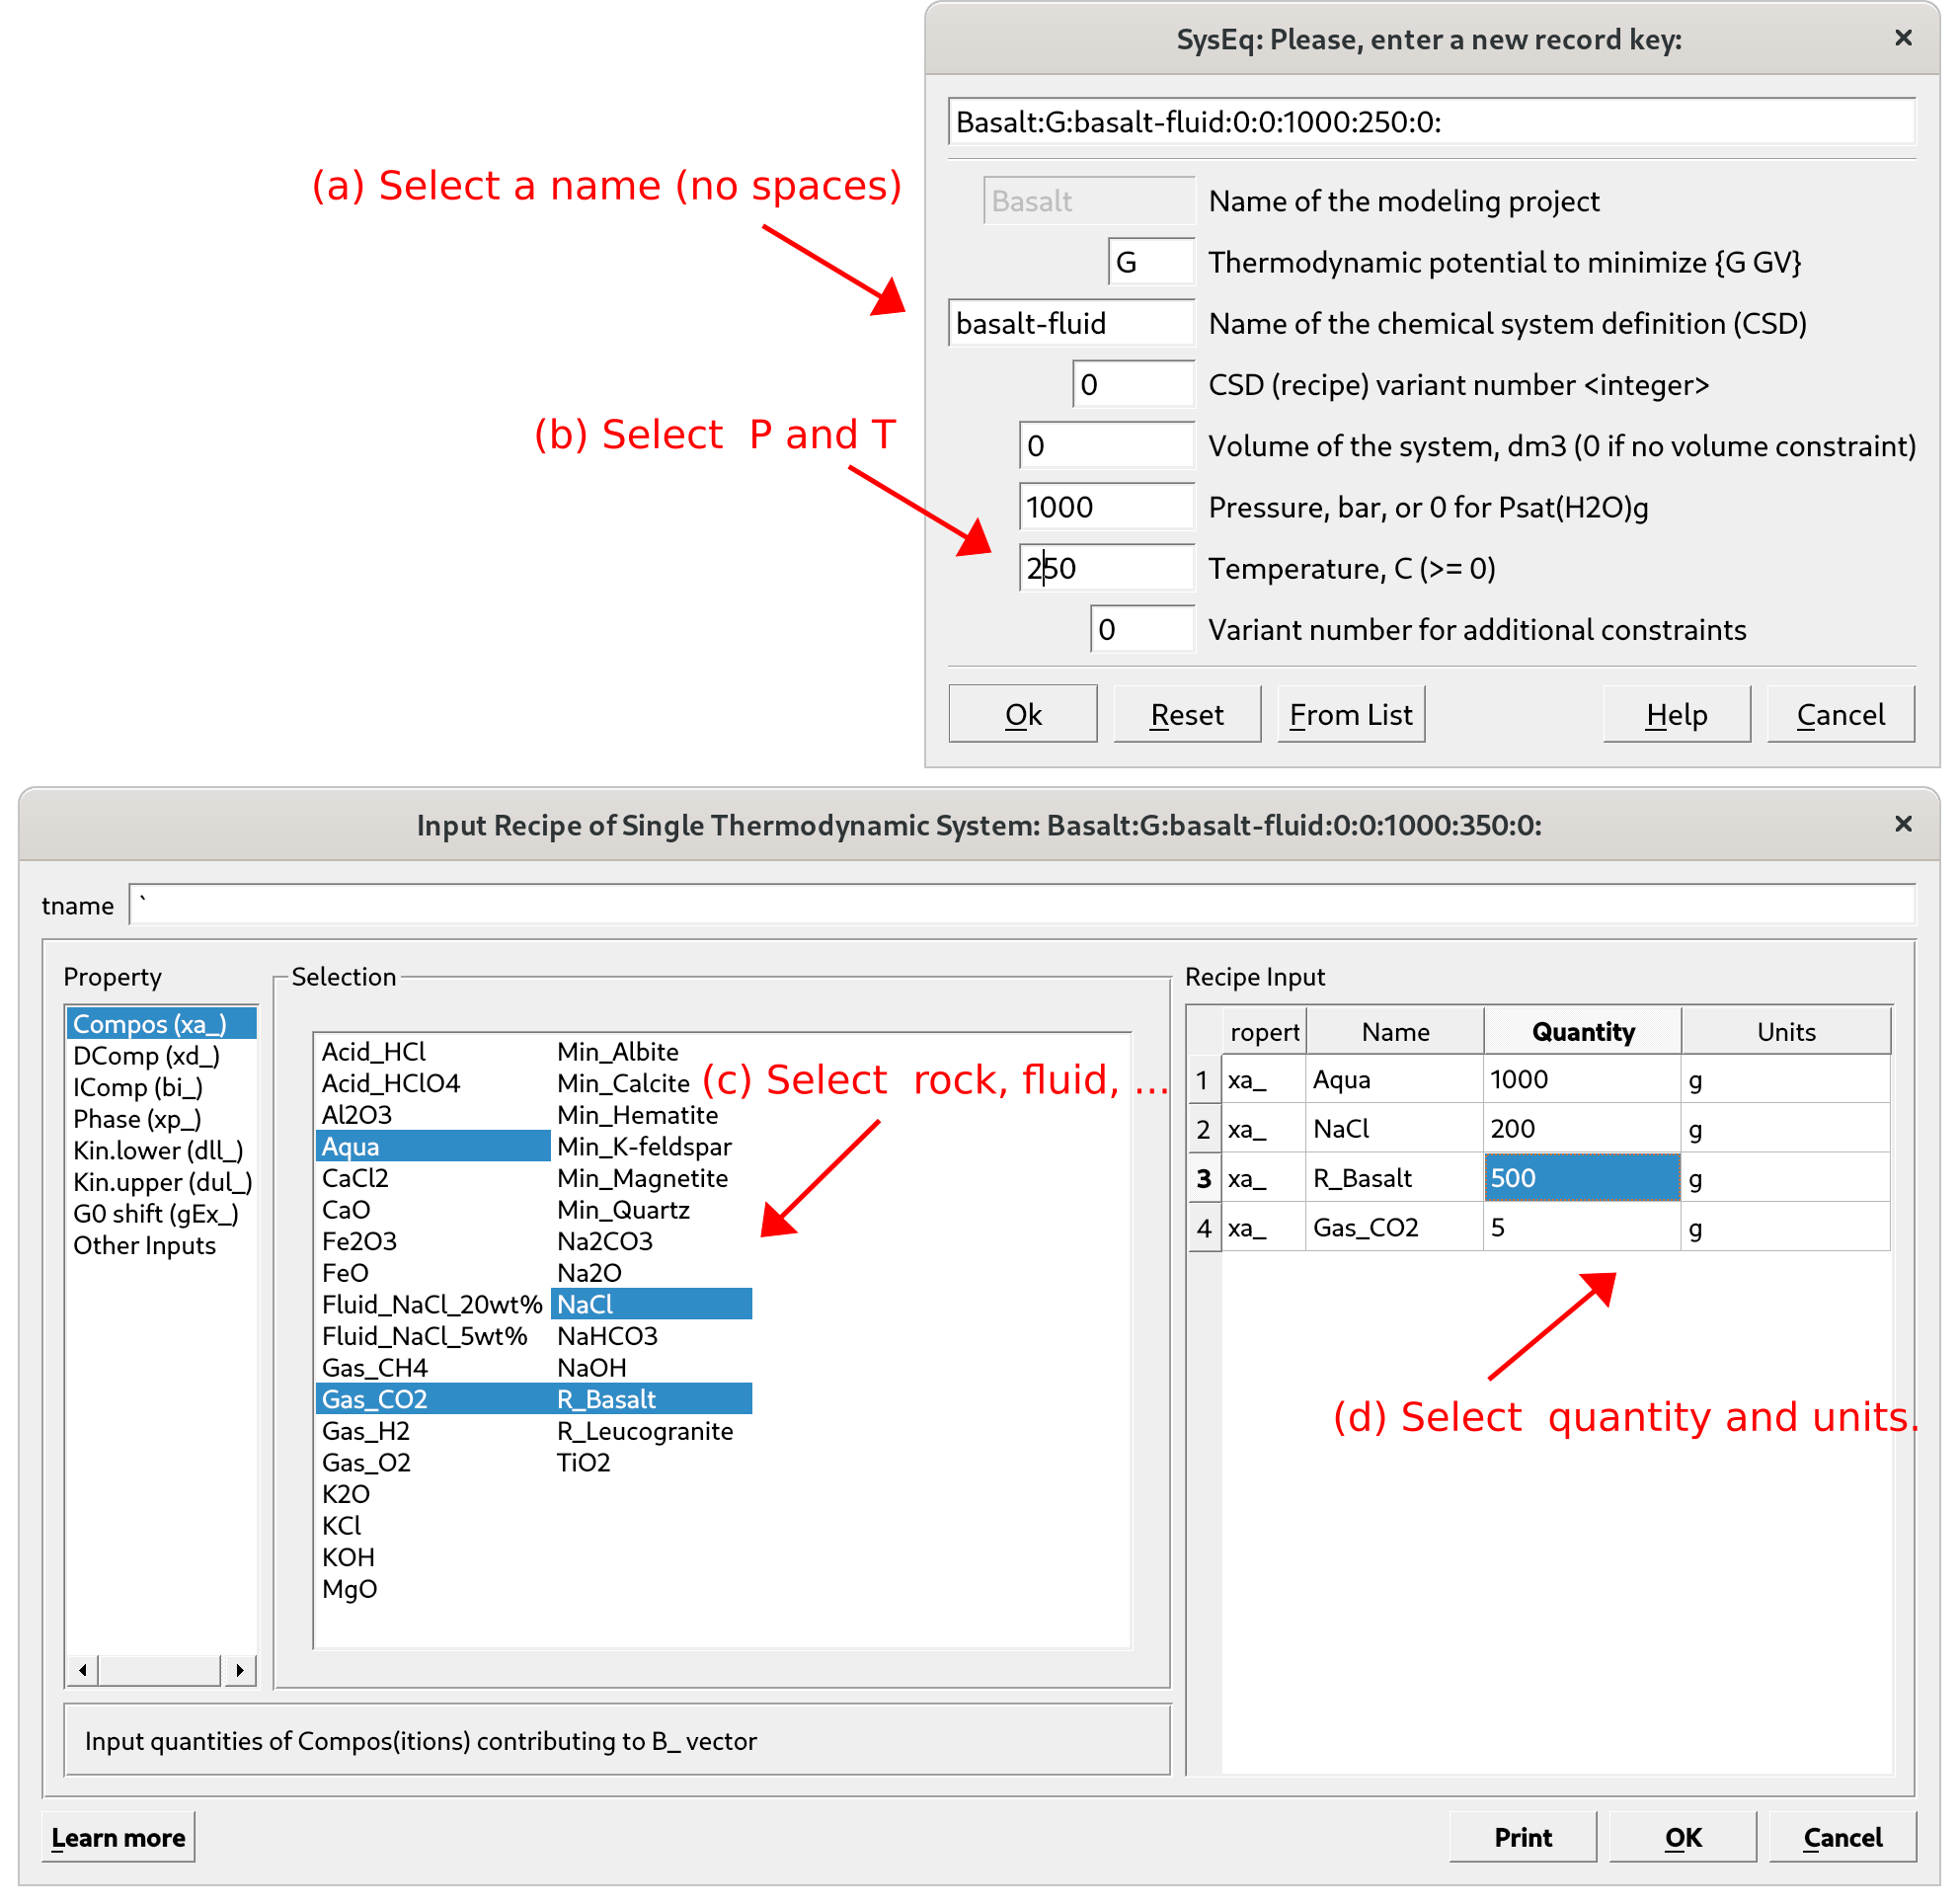
\includegraphics[width=0.7\linewidth]{figures/module1/fig-8} \caption{GEM-Selektor user interface showing the windows to create a new equilibrium system and define pressure (P) and temperature (T) for our first calculation.}\label{fig:fig-8}
\end{figure}

\begin{figure}
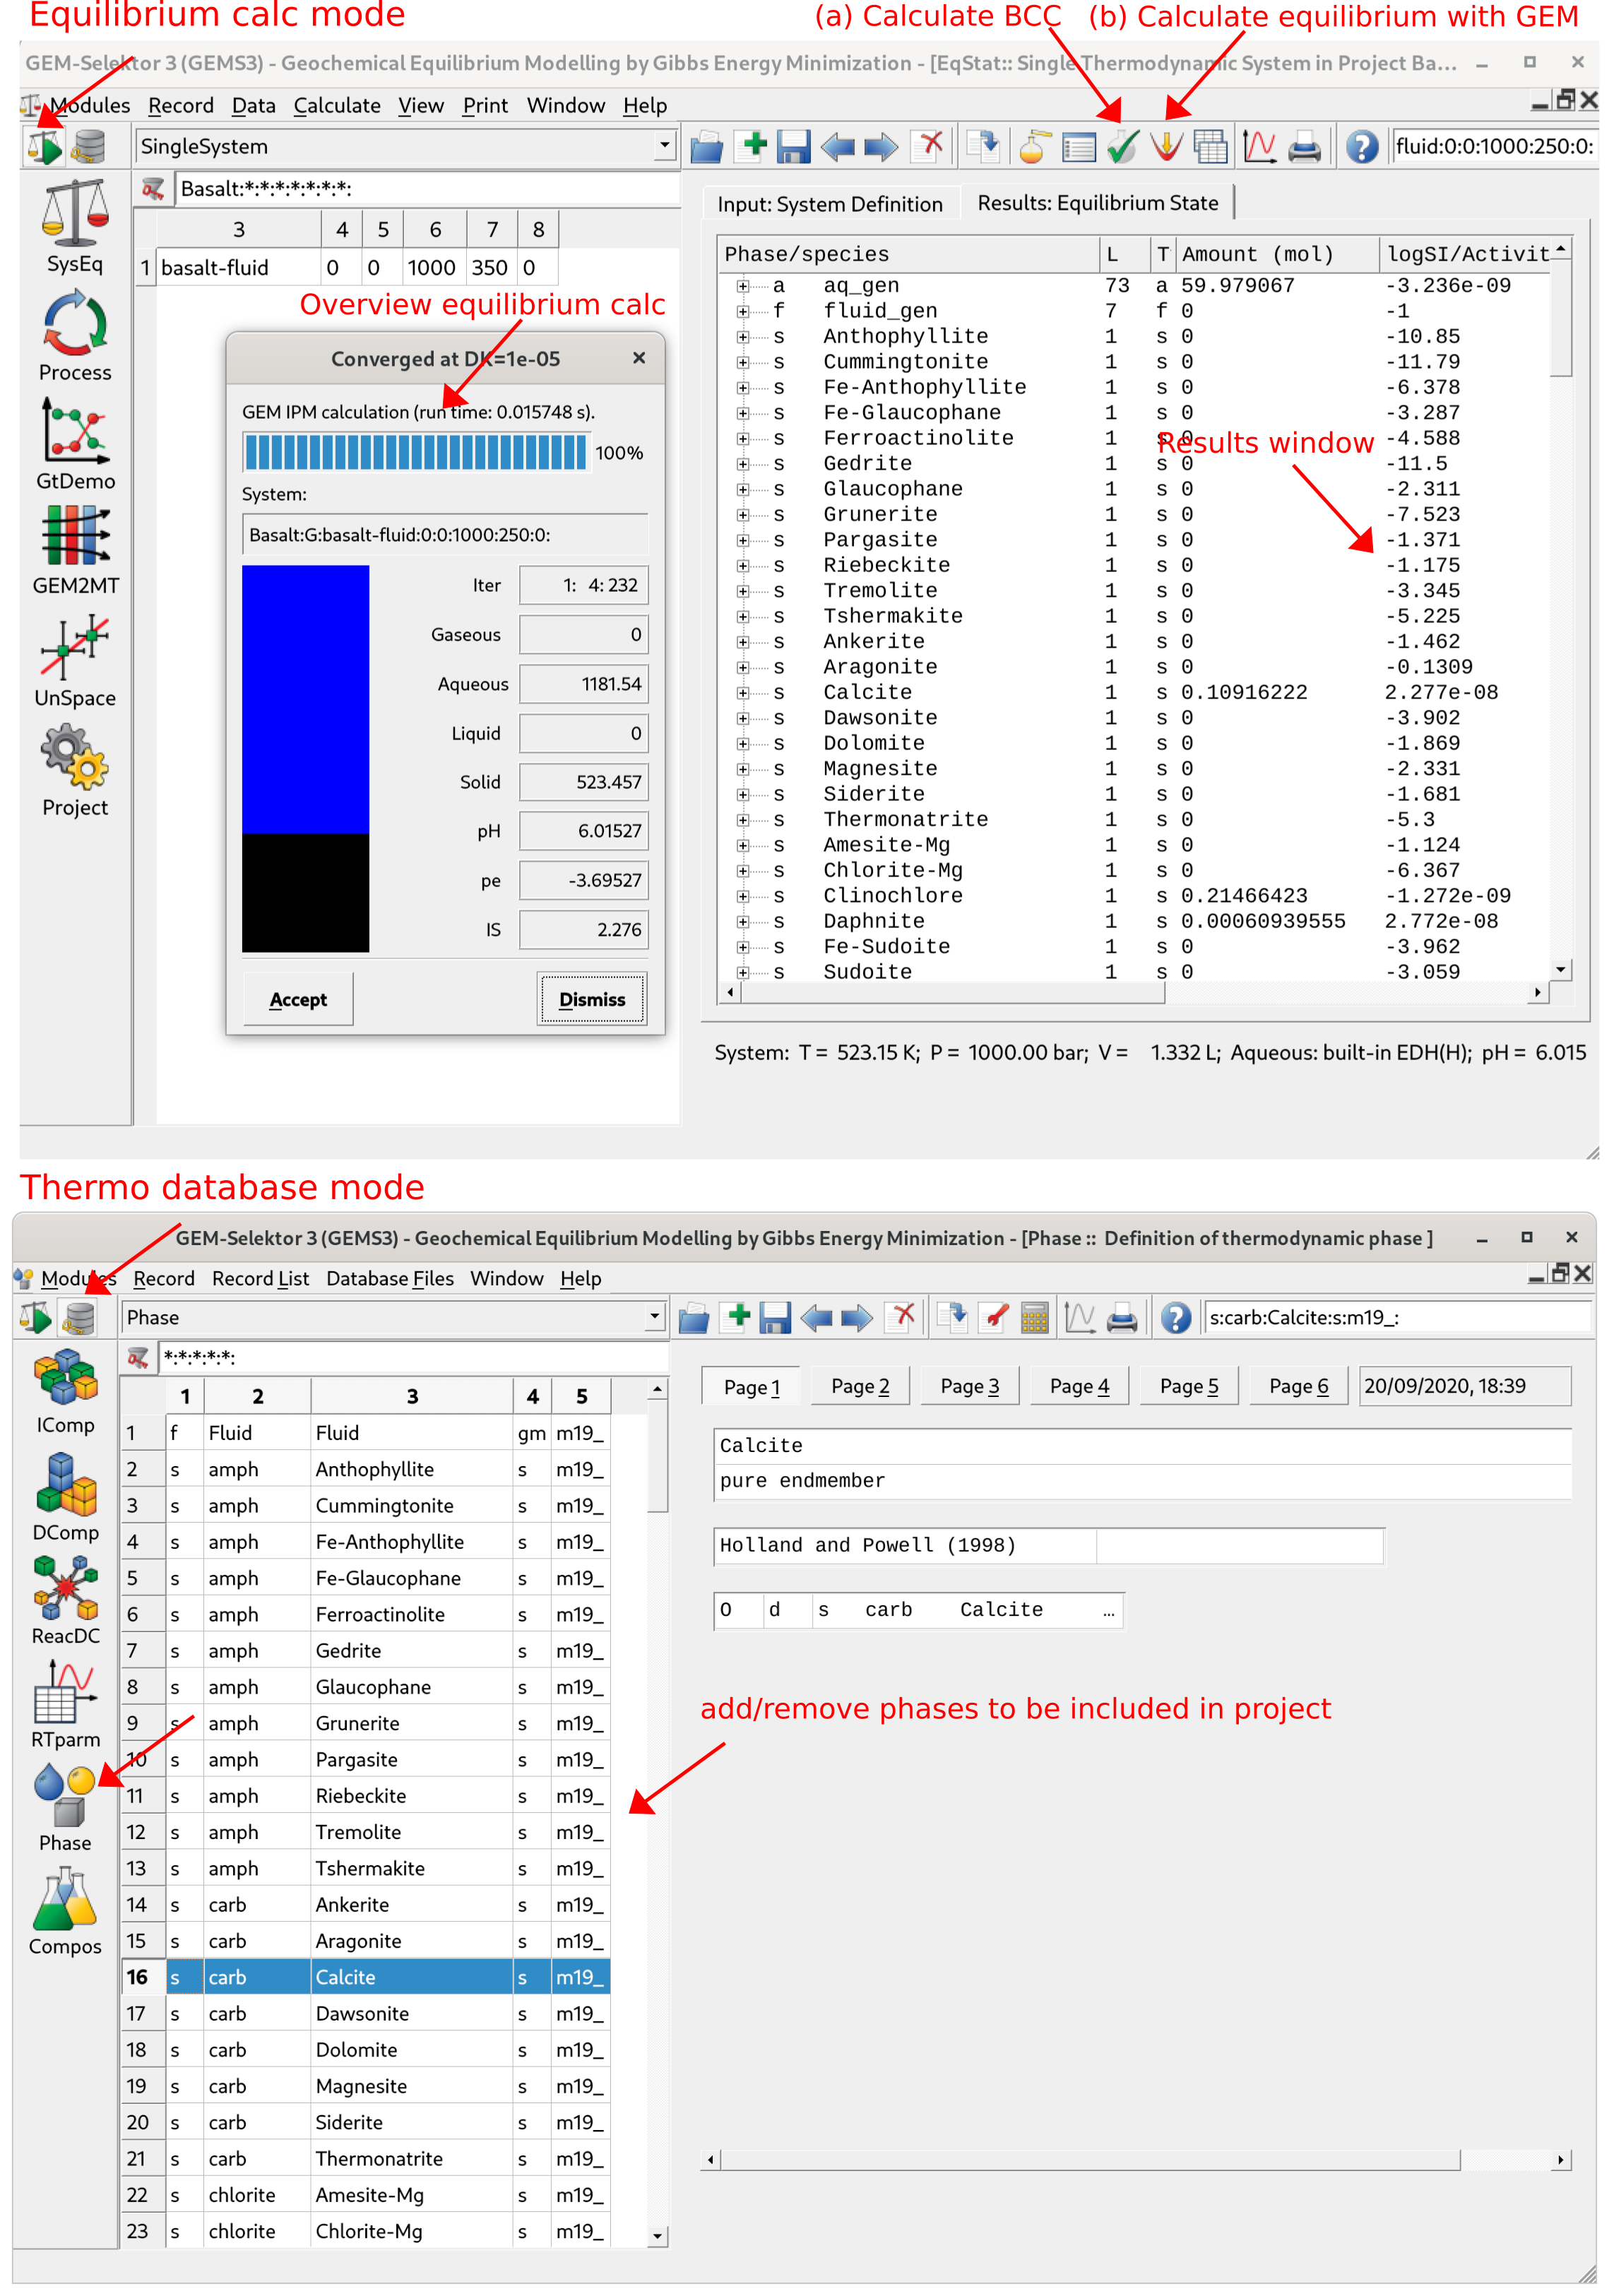
\includegraphics[width=0.7\linewidth]{figures/module1/fig-9} \caption{GEM-Selektor user interface showing how to `Calculate BCC` followed by `Calculate equilibrium with GEMS`. Also shown are the `Equilibrium Calculation` mode and the `Thermodynamic database` mode, where you can inspect the MINES database.}\label{fig:fig-9}
\end{figure}

\hypertarget{outcomes}{%
\section{Outcomes}\label{outcomes}}

Congratulations! In Module 1 you learned how to install the MINES thermodynamic database in your Resources/DB.default GEMS folder, the general folder structure of GEMS, how to setup your first project and how to run your first fluid-rock equilibrium calculations in GEMS.

\hypertarget{module2}{%
\chapter{Feldspar reaction path}\label{module2}}

In this tutorial, you will learn to model the reaction path of K-feldspar in contact with a NaCl-bearing aqueous solution and calculate the evolution of the fluid and the minerals formed as a function of increased fluid-rock interaction. You will also learn how to set up an automated cooling process simulation and plot results from multiple simulations. We will use the GEMS project file ``Module2'' that can be found either in the /Tutorial/Module2\_fsp-reaction/unsolved workshop folder or download it directly \href{https://geoinfo.nmt.edu/mines-tdb/GEMS-files/Module2.zip}{here}.

\hypertarget{compute-the-chemical-equilibrium-of-single-chemical-systems-syseq}{%
\section{Compute the chemical equilibrium of single chemical systems (SysEq)}\label{compute-the-chemical-equilibrium-of-single-chemical-systems-syseq}}

\begin{figure}
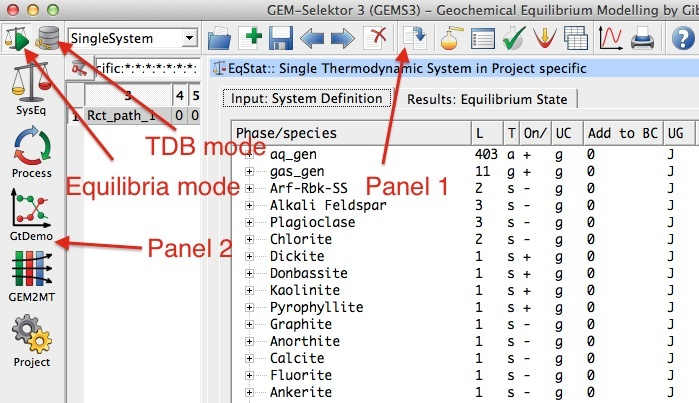
\includegraphics[width=0.7\linewidth]{figures/module2/fig-1} \caption{GEMS user interface showing the `Equilibria Calculation` and `Thermodynamic Database` modes.}\label{fig:fig-1b}
\end{figure}

\begin{itemize}
\item
  Copy the entire unzipped Module2 folder into your GEMS project directory located in Library/Gems3/projects. More information on the GEMS folder structure can be found in \protect\hyperlink{intro}{Module 1}.
\item
  Open GEMS and choose the project in the \texttt{Equilibria\ Calculation\ Mode}. The user interface is shown in Figure \ref{fig:fig-1b}. Panel 1 permits to create new records and run the program for calculations. Panel 2 gives you different calculation options.
\item
  Choose the \texttt{Create\ a\ new\ record\ from\ scratch} from the menu in Panel 1 and fill the parameters listed in Figure \ref{fig:fig-2b}
\item
  In the \texttt{Open\ recipe\ dialog}, which can also be found in Panel 1, add phases, quantity and units as shown in Figure \ref{fig:fig-3b}; Aqua (1000 g), HCl (0.1 M), NaCl (50 g), O\(_{2(g)}\) (1e-7) and K-feldspar (10 g).
\end{itemize}

\begin{figure}
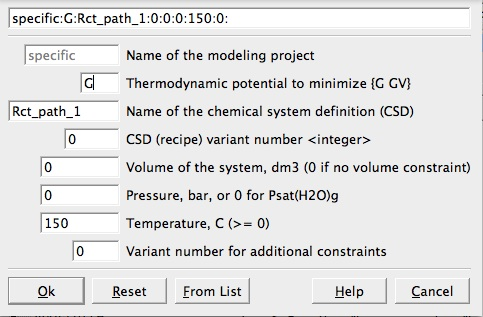
\includegraphics[width=0.7\linewidth]{figures/module2/fig-2} \caption{New record window. Select a name without spaces, a temperature and a pressure for your system. Note that a pressure of 0 corresond to saturated water vapor pressure.}\label{fig:fig-2b}
\end{figure}

\begin{figure}
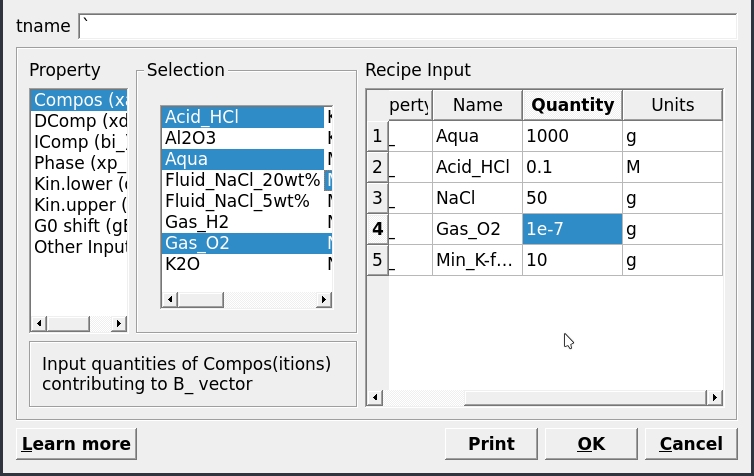
\includegraphics[width=0.7\linewidth]{figures/module2/fig-3} \caption{System recipe dialog.}\label{fig:fig-3b}
\end{figure}

\begin{itemize}
\item
  Model the chemical equilibrium between 10 g of K-feldspar (microcline) and H\(_2\)O at 150 \(^\circ\)C by pressing \texttt{Calculate\ BCC} followed by \texttt{Calculate\ Equilibrium} in Panel 1. Inspect the pop up window with pH, redox (eH) and phase proportions, then accept.

  -- Determine the pH of this system as shown in the lower right of the main window (Fig. \ref{fig:fig-4b}).

  -- What is the pH of this system with 10, 20, 50 and 100 g K-feldspar? Change the amount of feldspar by clicking the \texttt{Open\ recipe\ dialog} followed by \texttt{Calculate\ BCC} and by \texttt{Calculate\ Equilibrium}. What minerals are stable with increasing pH?
\item
  Finally, clone your existing Rct\_path\_1 chemical system by selecting it and choosing \texttt{Clone\ a\ new\ record\ from\ this\ one} in Panel 1 (Fig. \ref{fig:fig-1}). Change the name to Rct\_path\_2 and the temperature to 300 \(^\circ\)C in the pop up window, and recalculate the equilibrium of this system.

  -- Determine the pH of this system as shown in the lower right of the main window.

  -- What is the pH of this system with 10, 20, 50 and 100 g K-feldspar? What minerals are stable with increasing pH?

  -- Are there differences between the modeled system at 150 and 300 \(^\circ\)C
\end{itemize}

\begin{figure}
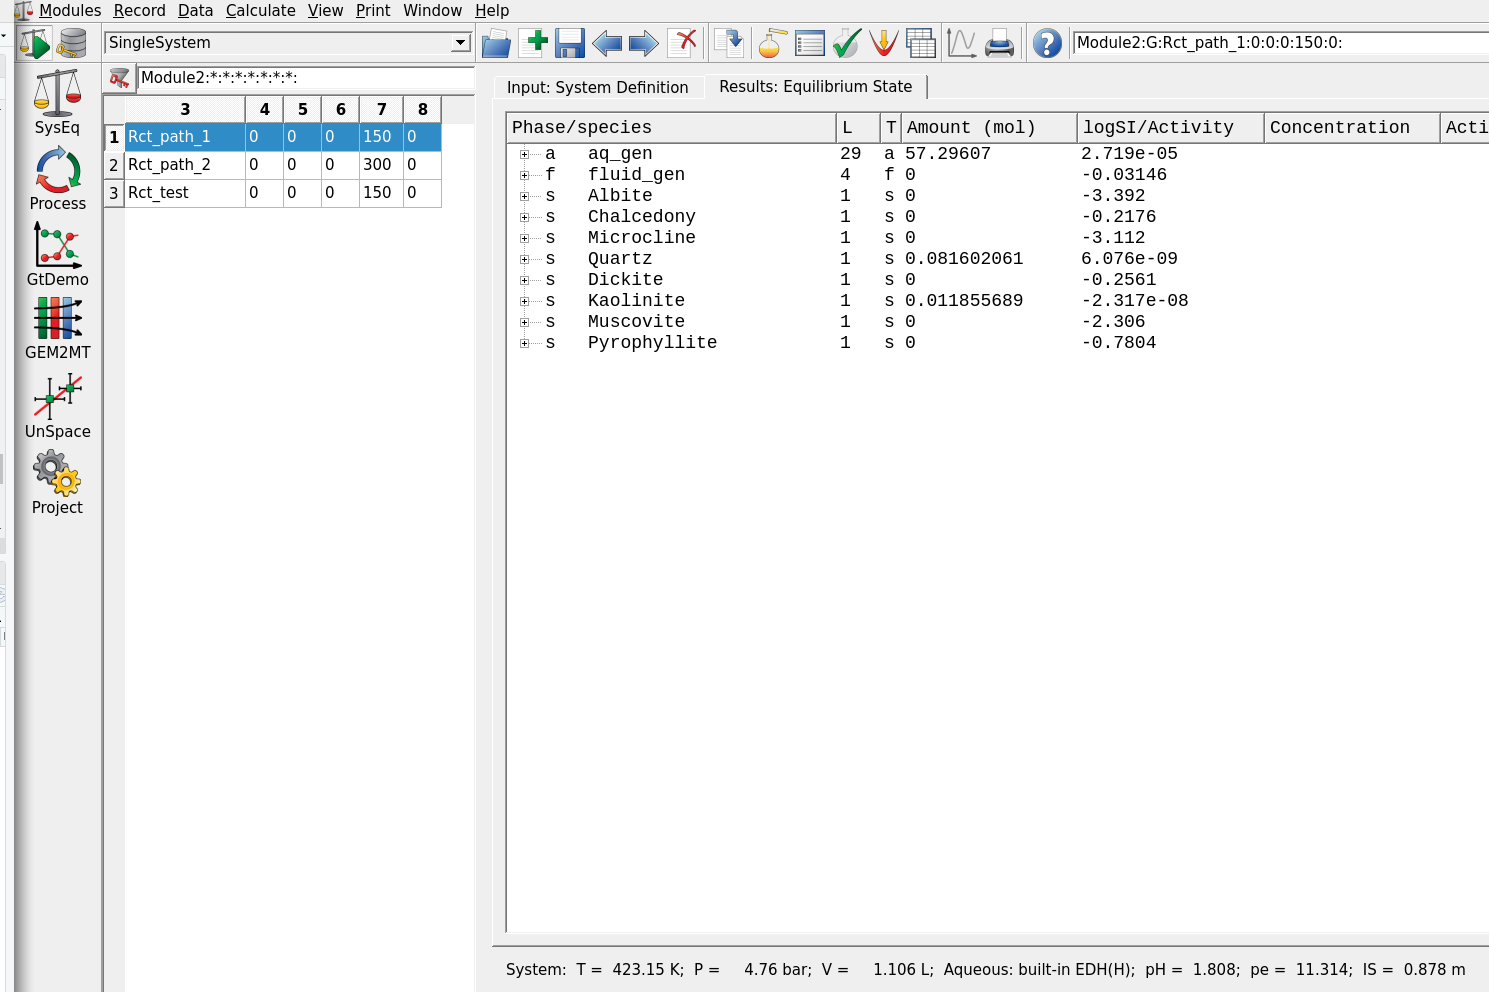
\includegraphics[width=0.9\linewidth]{figures/module2/fig-4} \caption{Results of the calculations, i.e. with 10 g K-feldspar added to the fluid.}\label{fig:fig-4b}
\end{figure}

\hypertarget{compute-processes-using-a-titration-model-process-s-mode}{%
\section{Compute processes using a titration model (Process, S mode)}\label{compute-processes-using-a-titration-model-process-s-mode}}

The previous part of this tutorial showed you how to do individual \texttt{SysEq} calculations. What if you want to automate this process and calculate the equilibria of 10 to 100 g feldspar in steps and plot the results, i.e.~a titration model? In the following we will see how to set up \texttt{Process} simulations.

\begin{itemize}
\item
  Select the \texttt{Process} option in Panel 2 (Fig. \ref{fig:fig-1b}).
\item
  Click \texttt{Create\ a\ record\ from\ scratch} in Panel 1 and select your parent chemical system \texttt{SysEq} calculated previously at 150 \(^\circ\)C (Fig. \ref{fig:fig-5b}).
\item
  Name this process simulation ``titration\_150C'' and use the \texttt{Process\ simulation\ code} (S) as shown in Figures \ref{fig:fig-6b}) and \ref{fig:fig-7b}).
\item
  In the next window, choose a model (\texttt{titration\ cNu\ linear}), a mineral ( \texttt{Compos}, Min\_K-feldspar) and select the temperature (150 \(^\circ\)C), pressure (0 for water vapor saturation P) and amount of mineral to be added (\texttt{iNu}: 10-250 g in 10 g steps) as shown in Figure \ref{fig:fig-8b}. The parameters are: set \texttt{iTm} 1000, 1200, 1; set \texttt{iP} to 0 all fields; set \texttt{iNu} 10, 250, 10, corresponding to start, end, and step values.
\item
  Select items to be plotted (\texttt{Scalars}: pH; \texttt{Xa}: Kaolinite, Pyrophyllite, Microcline, Muscovite, Albite and Quartz) as shown in Figure \ref{fig:fig-9b}.
\item
  Accept all the following dialogues. Then click on \texttt{Save\ this\ record\ to\ database} in Panel 1, which creates your new process simulation record. Then click on the calculator icon \texttt{Re-calculate\ and\ check\ record\ data} without displaying the graph.
\end{itemize}

\begin{figure}
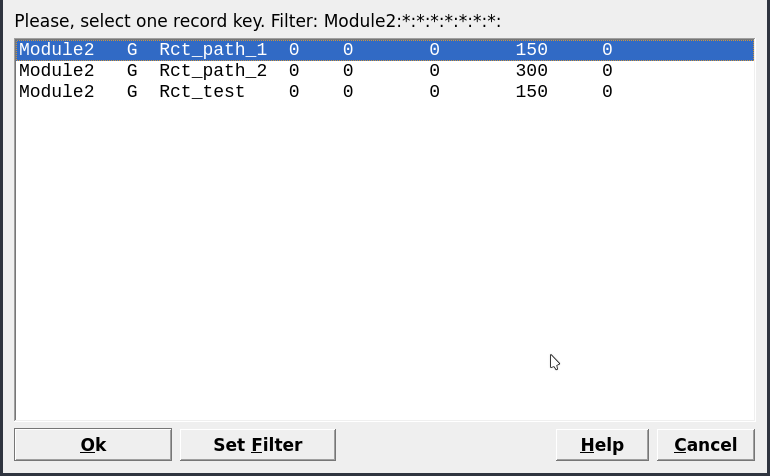
\includegraphics[width=0.7\linewidth]{figures/module2/fig-5} \caption{Select a parent chemical system (`SysEq`) for modeling a `Process`.}\label{fig:fig-5b}
\end{figure}
\begin{figure}
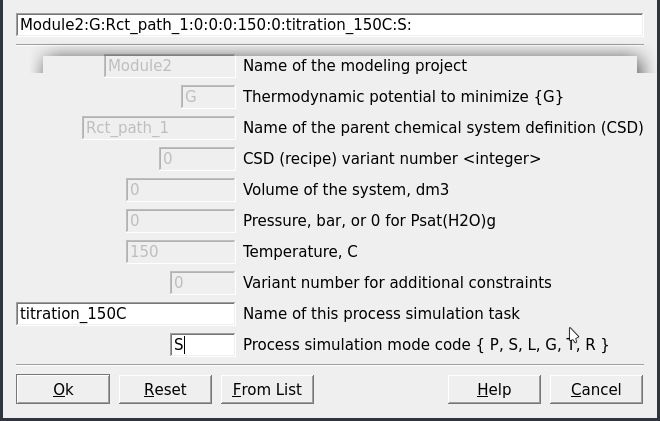
\includegraphics[width=0.7\linewidth]{figures/module2/fig-6} \caption{Name the `Process` simulator and indicate the model type (note: the process type code names are described and changeable on the next screen as well).}\label{fig:fig-6b}
\end{figure}

\begin{figure}
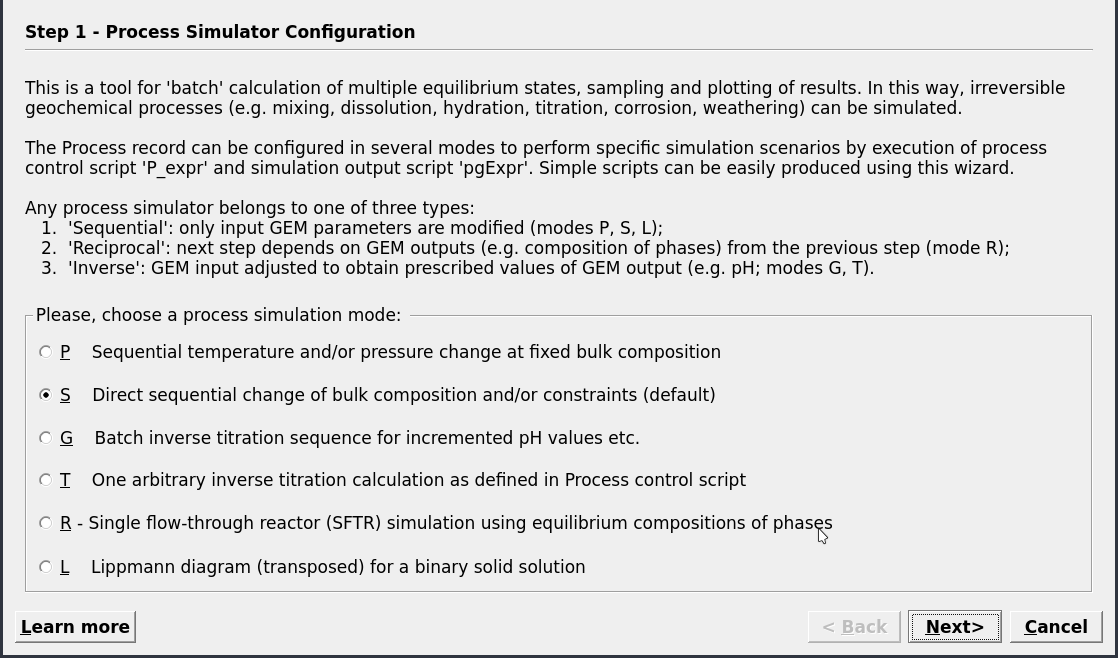
\includegraphics[width=0.9\linewidth]{figures/module2/fig-7} \caption{Window showing the different simulations types. Module 2 covers `mode S` for titration  or `mode P` for cooling/heating models.}\label{fig:fig-7b}
\end{figure}
\begin{figure}
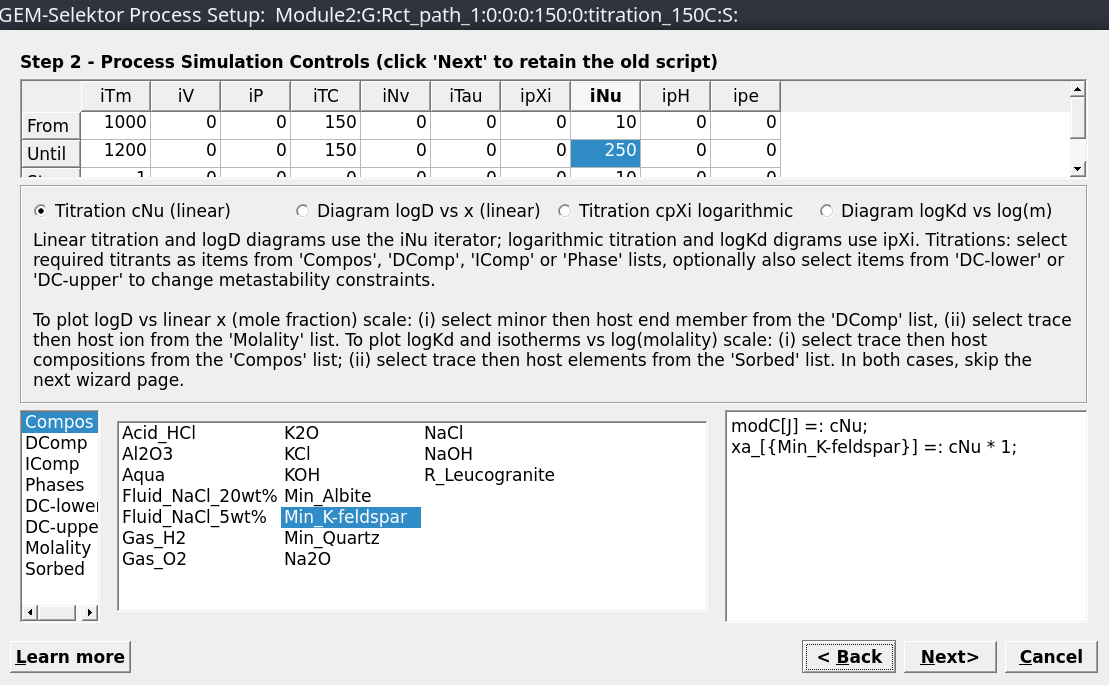
\includegraphics[width=0.9\linewidth]{figures/module2/fig-8} \caption{Set the parameters for the `Process` simulation; Set `iTm` 1000, 1200, 1; Set `iP` to 0 all fields; Set `iNu` 10, 250, 10.}\label{fig:fig-8b}
\end{figure}

\begin{figure}
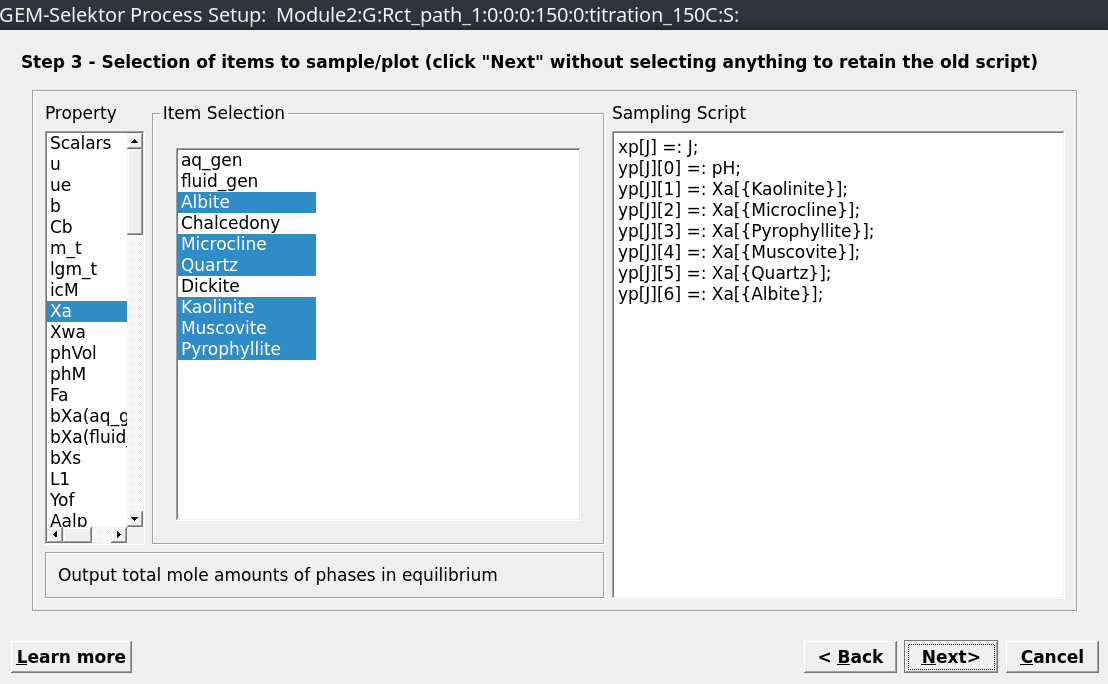
\includegraphics[width=0.9\linewidth]{figures/module2/fig-9} \caption{Choose the results to be plotted, including pH and mole minerals.}\label{fig:fig-9b}
\end{figure}

\begin{itemize}
\item
  There is a tab menu with 3 important selections: \texttt{Controls}, \texttt{Sampling} and \texttt{Results}. In the \texttt{Controls} tab add a description of the modeling project (Fig. \ref{fig:fig-10b}). In the \texttt{Sampling} tab change the script as shown in Figure \ref{fig:fig-11b} to choose as x-variable the amount of K-feldspar added (the process extent variable \texttt{cNu}).
\item
  Click \texttt{Save\ this\ record\ to\ database}. Toggle to the \texttt{Results} tab to inspect your modeling results. Then click on the calculator icon \texttt{Re-calculate\ and\ check\ record\ data} and check what happens with the column xp. You just assigned the \texttt{cNu} variable to the x-axis and GEMS registered it. If not, go back on the \texttt{Sampling} tab and check your script! Now lets inspect the results\ldots{}

  -- How many grams of K-feldspar need to be added to get a constant pH and what is the value?

  -- Which mineral assemblages buffer the fluid pH and can pH ranges be distinguished?
\end{itemize}

\begin{figure}
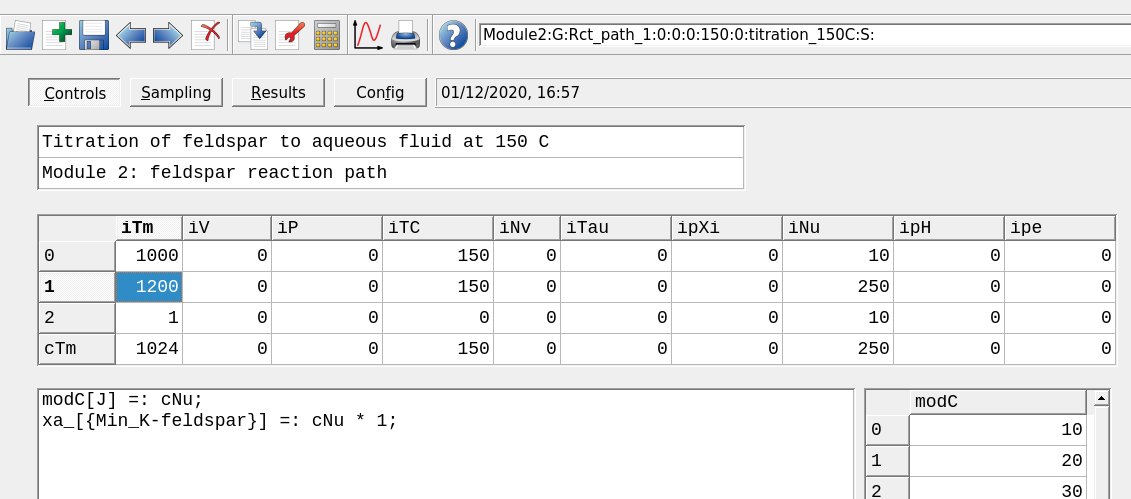
\includegraphics[width=1\linewidth]{figures/module2/fig-10} \caption{The `Controls` window showing the model conditions. The top dialog is used to add a comment and the script dialog can be customized. `iTm` is used to set the record variable; `iP` to set pressure and `iTC` temperature; `iNu` is the process variable, in this case the amount of feldspar.}\label{fig:fig-10b}
\end{figure}

\begin{figure}
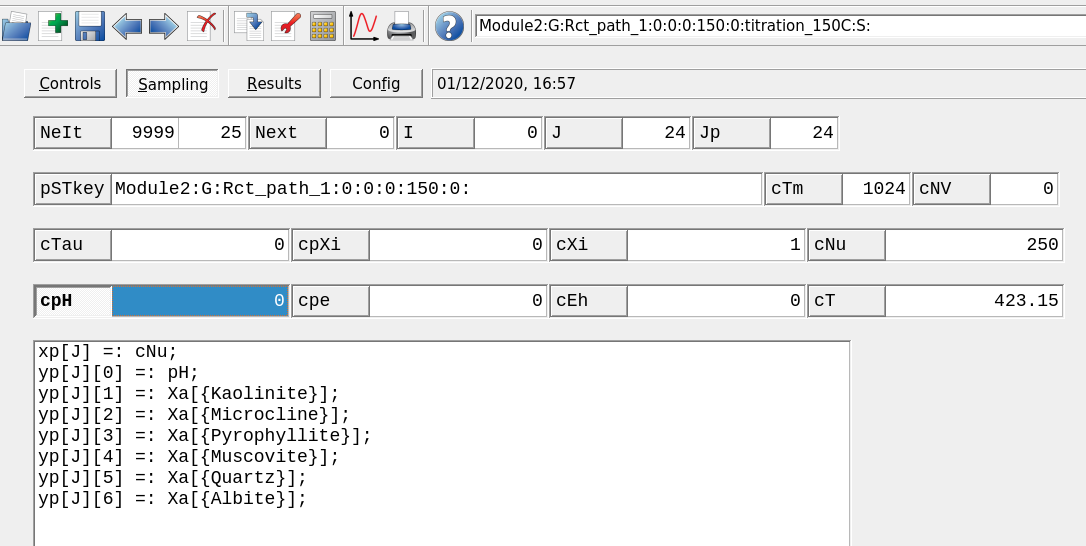
\includegraphics[width=1\linewidth]{figures/module2/fig-11} \caption{The `Sampling` window showing the x- and y-axes to be sampled. Make sure to change `xp[J]` to `cNu` which is the progress variable. Then click on a blank space to make sure the script window has been registered followed by `Save this record in the database` in the top panel.}\label{fig:fig-11b}
\end{figure}

\hypertarget{change-p-t-of-the-titration-model}{%
\section{Change P-T of the titration model}\label{change-p-t-of-the-titration-model}}

Now lets clone our record to calculate the exact same titration model but changing the temperature (T) to 300 \(^\circ\)C and the pressure (P) to 500 bar.

\begin{itemize}
\item
  Clone your existing process simulation by selecting the existing record on the left and choose \texttt{Clone\ a\ new\ record}, then select your \texttt{SysEq} parent system calculated at 300 \(^\circ\)C (Fig. \ref{fig:fig-12b}). Accept all the following dialogues.
\item
  In the \texttt{Controls} tab change the description of the modeling project and change the temperature to 300 \(^\circ\)C and pressure to 500 bar to replace the starting and ending values (Fig. \ref{fig:fig-13b}). Click \texttt{Save\ this\ record\ to\ database}.
\item
  Switch the tab to \texttt{Results} and click the calculator icon \texttt{Re-calculate\ and\ check\ record\ data} to see how the pH values and moles minerals are changed by increasing the system temperature.
\item
  Toggle between both calculated process simulations at 150 and 300 \(^\circ\)C on the left pane and compare the results.
\end{itemize}

\begin{figure}
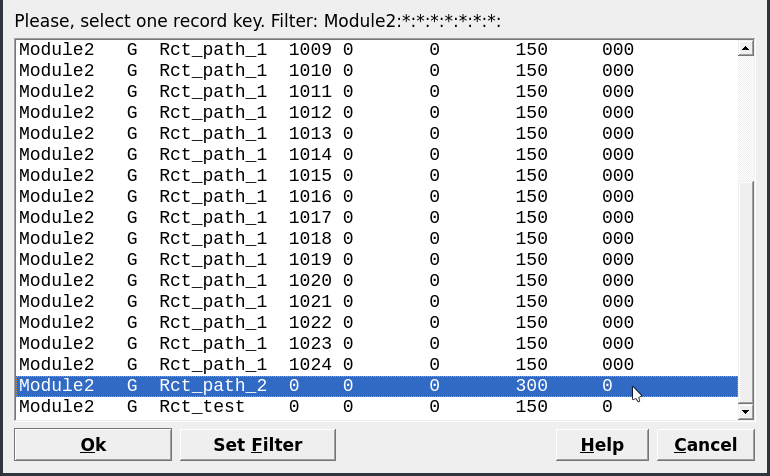
\includegraphics[width=0.7\linewidth]{figures/module2/fig-12} \caption{The `Sampling` window showing the x- and y-axes to be sampled. Make sure to change `xp[J]` to `cNu` which is the progress variable. Then click on a blank space to make sure the script window has been registered followed by `Save this record in the database` in the top panel.}\label{fig:fig-12b}
\end{figure}

\begin{figure}
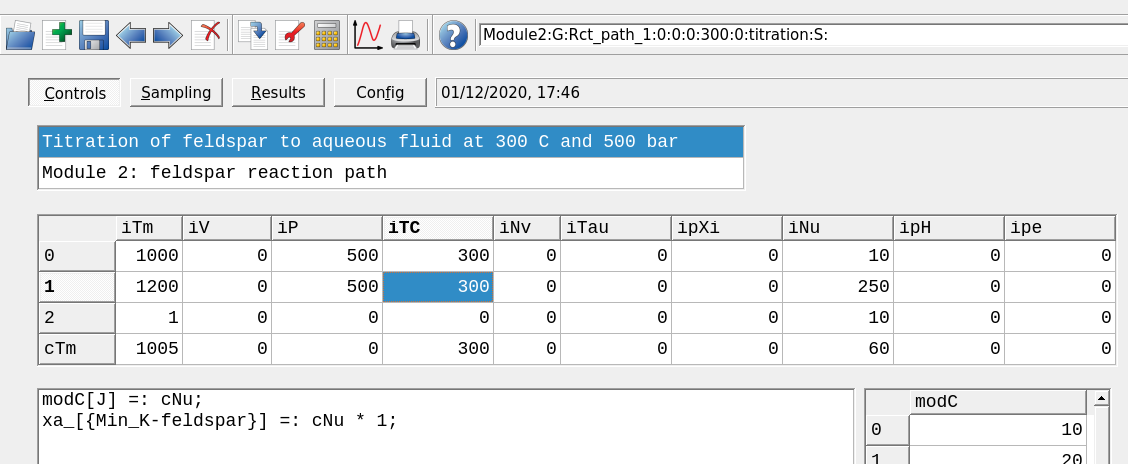
\includegraphics[width=0.8\linewidth]{figures/module2/fig-13} \caption{The `Controls` window showing a model set up at a different temperture and pressure.}\label{fig:fig-13b}
\end{figure}

\hypertarget{tweak-and-plot-the-results}{%
\section{Tweak and plot the results}\label{tweak-and-plot-the-results}}

What are the main differences for the simulations at 150 vs.~300 \(^\circ\)C? To make a better comparison lets fine tune the models and plot them!

\begin{itemize}
\item
  Select the process simulation you generated previously at 150 \(^\circ\)C and in the \texttt{Controls} tab change the amount of K-feldspar to be added using 2 to 50 g in 2 g steps and save.
\item
  Choose the \texttt{Results} tab and click the calculator icon \texttt{Re-calculate\ and\ check\ record\ data}. Click on the small \texttt{Plot\ data\ on\ Graph\ dialog} in Panel 1. The resulting graph should look similar to Figure \ref{fig:fig-14b}. The plots indicate different mineral assemblage buffer the fluid at different pH values. You can inspect which minerals by choosing the Customize button with values shown in \autoref{fig:process1h.jpeg}.
\end{itemize}

-- The resulting reaction path at 150 \(^\circ\)C is shown in \autoref{fig:process1i.jpeg}.

-- The resulting reaction path at 300 \(^\circ\)C is shown in \autoref{fig:process1j.jpeg}

\begin{figure}
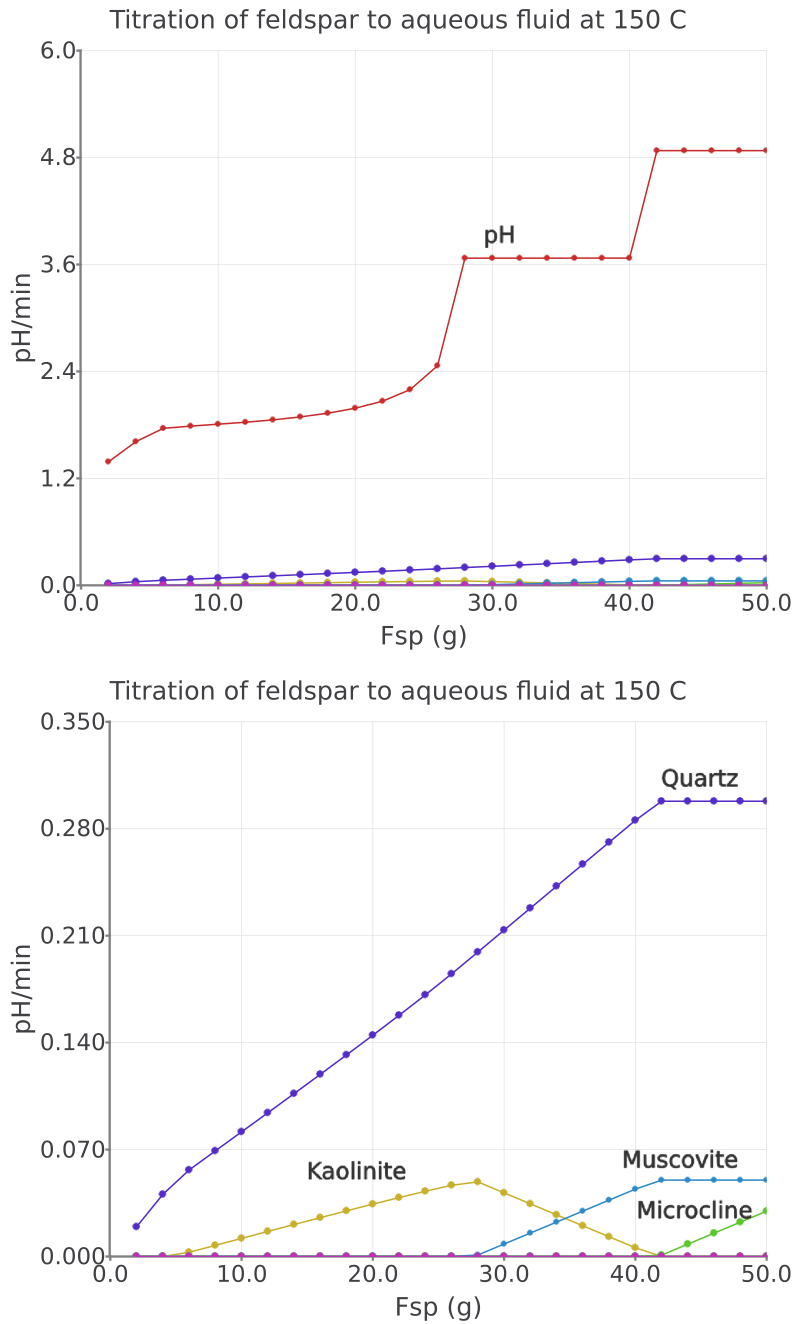
\includegraphics[width=0.8\linewidth]{figures/module2/fig-14} \caption{Simulated K-feldspar reaction path show pH and moles minerals in equilibrium with a saline aqueous fluid at 150 °C and saturated water vapor pressure.}\label{fig:fig-14b}
\end{figure}

\hypertarget{compute-processes-using-a-cooling-model-process-p-mode}{%
\section{Compute processes using a cooling model (Process, P mode)}\label{compute-processes-using-a-cooling-model-process-p-mode}}

Or what if you want to calculate the equilibria between feldspar and the aqueous fluid at 150 to 250 \(^\circ\)C in steps, i.e.~a cooling model?

\hypertarget{module-3}{%
\chapter{Module 3}\label{module-3}}

Work in progress\ldots{}

\hypertarget{module-4}{%
\chapter{Module 4}\label{module-4}}

Work in progress\ldots{}

\hypertarget{module-5}{%
\chapter{Module 5}\label{module-5}}

Work in progress\ldots{}

  \bibliography{book.bib,packages.bib}

\end{document}
